%=======================================================================
% Template para projeto de pesquisa/desenvolvimento
% Bacharelado em Sistemas de Informação  Universidade Federal  Rural de Pernambuco
%=======================================================================

\documentclass[a4paper,12pt,oneside]{article}

%% --- Codificação e idioma ---
\usepackage[T1]{fontenc}
\usepackage[utf8]{inputenc}
\usepackage[brazil]{babel}

%% --- Fontes ---
\usepackage{lmodern}
\usepackage{microtype}

%% --- Geometria e espaçamento (padrão ABNT NBR 14724) ---
\usepackage[a4paper,
            top=3.0cm, bottom=2.0cm,
            left=3.0cm, right=2.0cm]{geometry}
\usepackage{setspace}
\onehalfspacing
%espaçamento entre parágrafos
\setlength{\parindent}{.0in}
\parskip 10pt

%% The amssymb package provides various useful mathematical symbols
\usepackage{amssymb}
%% The amsthm package provides extended theorem environments
\usepackage{amsthm}
\usepackage{amsmath}
\usepackage[hidelinks]{hyperref}
\newcommand{\D}{\displaystyle}
\newcommand{\mc}{\multicolumn}
\newcommand{\ft}{\footnotesize}
\newcommand{\Sc}{\scriptsize}
\newcommand{\rset}{\mathbb{R}}
\newcommand{\zset}{\mathbb{Z}}
\newcommand\SB[1]{{\color{cyan} #1}}
\newcommand{\HRule}{\rule{\linewidth}{0.5mm}}
\usepackage{color}
\usepackage{graphicx}
\usepackage{url}
\usepackage{xurl}
\usepackage{appendix}
\usepackage{booktabs}
\usepackage{array}
% Coluna de largura fixa alinhada à esquerda, para tabelas com texto.
\newcolumntype{L}[1]{>{\raggedright\arraybackslash}p{#1}}

% O logotipo fica em figures/ e as figuras do estudo são geradas em ../figures/.
\graphicspath{{figures/}{../figures/}}

%% --- Bibliografia ABNT ---
\usepackage[alf,abnt-emphasize=bf,bibjustif,abnt-etal-list=0]{abntex2cite}

%% --- Cabeçalho/rodapé com filete UFRPE ---
\usepackage{fancyhdr}
\setlength{\headheight}{24.1pt}
\pagestyle{fancy}
\fancyhf{}
\rhead{\small{Projeto de Pesquisa, UFRPE}}
\cfoot{\thepage}
\renewcommand{\headrulewidth}{1.2pt}
\renewcommand{\headrule}{\hbox to\headwidth{%
  \leaders\hrule height \headrulewidth\hfill}}



% inicio do documento
\pagestyle {empty}
\begin{document}
\begin{center}

%início da capa


\includegraphics[width=0.2\textwidth]{figures/logoufrpe.jpg}\\[0.2cm]


{\large \bf{Universidade Federal Rural de Pernambuco}} \\
Bacharelado em Sistemas de Informação \\
 Departamento de Estatística e Informática

\vspace{0.0cm}
\noindent
% identificação do trabalho
\HRule \\[0.4cm]
{\large \bfseries Proposta de Projeto \\[0.3cm]
Modelo hospedeiro e vetor com período de latência para o monitoramento da chikungunya no Recife
 \\[0.4cm]}
\HRule
\\[1.0cm]

% identificação do líder da Equipe
\large\textbf{Líder}\\
Leandro Cesar\\[1cm]

% identificação do orientador
\large\textbf{Orientadora}\\
Silvana Bocanegra\\
Departamento de Estatística e Informática\\[1cm]

\vfill

{\large {\bf Recife}\\
Outubro de 2026}
\end{center}

\begin{abstract}
A chikungunya é uma arbovirose transmitida pelo \textit{Aedes aegypti} que deixa dor articular crônica em
grande parte dos infectados. O Recife teve duas epidemias, em 2015 e 2016 e em 2021, e um inquérito
sorológico de 2018 e 2019 mostrou que cerca de 64\% da população ainda não havia sido infectada. Esta
proposta tem como objetivo desenvolver e calibrar um modelo compartimental SEIR-SEI, com períodos de
latência no humano e no mosquito e o vetor como população explícita, para o monitoramento da chikungunya
no Recife. O ponto de partida é um modelo SIR, revisado e conferido contra suas expressões analíticas, cujas
limitações foram medidas com dados reais: com o número de reprodução da literatura, o SIR prevê 96\% de
infectados e o pico 38 dias após o primeiro caso, enquanto o inquérito mediu 36\% e a primeira onda levou
cerca de seis meses até o pico. O SEIR-SEI, já implementado, leva o pico para cerca de nove meses com o
mesmo número de reprodução, e a taxa de crescimento observada nas notificações implica números de
reprodução diferentes em cada modelo, o que mostra que a estrutura do modelo importa para ler os dados.
Comparados com nove pontos observados, o SIR diverge em seis e o SEIR-SEI em cinco. A onda de 2021 cresceu
2,2 vezes mais rápido que a primeira, na estação chuvosa, e se distribuiu de outro modo entre os
distritos, o que aponta a sazonalidade e a heterogeneidade como os componentes que faltam.
O projeto vai calibrar o SEIR-SEI com as notificações de 2015 a 2025 do portal de dados abertos da
Prefeitura, usando o inquérito sorológico como restrição, incluir sazonalidade e heterogeneidade entre
grupos da cidade e avaliar cenários de controle vetorial. Os produtos esperados são o modelo calibrado,
estimativas da imunidade remanescente e um repositório aberto e reprodutível.

{\raggedright\textbf{Palavras-chave:} chikungunya; modelo compartimental; SEIR-SEI; \textit{Aedes aegypti};
Recife.\par}
\end{abstract}

\pagestyle {fancy}
\tableofcontents

\setcounter{page}{0} \pagenumbering{arabic}
\section{Apresentação}
\label{sec:apresentacao}

A chikungunya é uma doença causada por um vírus transmitido principalmente pelo mosquito \textit{Aedes
aegypti}. Depois de uma incubação de alguns dias, provoca febre e dor articular intensa \cite{who2025}.
Em parte dos pacientes a dor persiste: numa revisão sistemática, 43\% dos infectados não estavam
recuperados três meses depois da infecção \cite{paixao2018}. Isso faz da doença um problema que dura muito
além do surto, com impacto sobre o trabalho das pessoas e sobre os serviços de saúde.

O vírus chegou ao Brasil em 2014. Entre 2013 e 2022 foram registrados 253.545 casos confirmados em
laboratório, em sete ondas epidêmicas, com o Nordeste como região mais atingida \cite{desouza2023}. No
Recife, as notificações do portal de dados abertos da Prefeitura \cite{recife2026} mostram duas grandes
ondas. A primeira começou em agosto de 2015 e teve pico na semana de 14 de fevereiro de 2016, com 9.989
casos prováveis em 2015 e 2016. A segunda, em 2021, foi ainda maior nas notificações, com 16.013 casos
prováveis. Um inquérito domiciliar feito na cidade entre 2018 e 2019 encontrou anticorpos contra o vírus
em 35,7\% da população \cite{braga2023}. Ou seja, cerca de dois terços dos moradores ainda podiam se
infectar.

A vigilância conta casos, mas os casos notificados são uma fração pequena das infecções. Comparando a
sorologia com as notificações, há cerca de 53 infecções para cada caso provável notificado na primeira
onda. Os casos também não dizem, sozinhos, quanta imunidade a cidade já acumulou nem quanto uma campanha
contra o mosquito pode reduzir a próxima onda. Para responder a essas perguntas é preciso um modelo que
represente o ciclo de transmissão.

Este projeto parte de um trabalho anterior da disciplina, em que um modelo SIR clássico foi aplicado à
introdução da chikungunya no Recife. O SIR foi revisado e conferido contra suas expressões analíticas, e
suas distâncias em relação aos dados foram medidas: ele prevê que 96\% da população se infecte e põe o pico
38 dias depois do primeiro caso, enquanto o inquérito mediu 36\% e a primeira onda levou cerca de seis meses
até o pico. As causas dessas distâncias são conhecidas. O SIR não tem o mosquito, não tem o período de
latência e supõe que toda a cidade se mistura de forma homogênea.

A proposta é desenvolver um modelo SEIR-SEI, com períodos de latência no humano e no mosquito e o vetor
como população explícita, calibrá-lo com as notificações do Recife e com o inquérito sorológico, e usá-lo para monitorar
a transmissão e avaliar cenários de controle vetorial.

\section{Relevância}
\label{sec:relevancia}

A chikungunya continua circulando no Brasil em ondas recorrentes \cite{desouza2023}, e no Recife a maior
parte da população ainda é suscetível \cite{braga2023}. Como a forma crônica da doença é frequente
\cite{paixao2018}, cada nova onda deixa um número grande de pessoas com dor articular por meses. Saber
quanta imunidade a cidade acumulou, em que ritmo a transmissão cresce e quando uma ação contra o mosquito
ainda faz diferença é útil para a vigilância e para o planejamento do controle vetorial.

Três argumentos justificam o projeto agora.

\textbf{Maturidade técnica.} Pela primeira vez há, para o Recife, uma série pública de notificações de
chikungunya por semana e por bairro, de 2015 a 2025 \cite{recife2026}, e um inquérito sorológico de base
populacional \cite{braga2023}. A série permite ajustar a dinâmica do modelo, e o inquérito fixa quantas
pessoas foram de fato infectadas, o que separa a transmissão da subnotificação. As ferramentas para
integrar e ajustar modelos de equações diferenciais são abertas e maduras \cite{rcore2025, soetaert2010}.

\textbf{Capacidade local.} Os resultados preliminares já incluem o tratamento reprodutível dos dados do
portal, um modelo SIR conferido contra todas as suas expressões analíticas e o modelo SEIR-SEI
implementado e verificado contra a teoria (Seção \ref{sec:preliminares}). O projeto começa com a base
pronta.

\textbf{Impacto esperado.} O modelo calibrado vai produzir estimativas da imunidade remanescente e cenários
de controle vetorial para a cidade, em código aberto que pode ser atualizado com as notificações de cada
ano. Sistemas como o InfoDengue já estimam a transmissão a partir das notificações \cite{codeco2018}. A
contribuição deste projeto é complementar: um modelo mecanístico, com o mosquito e a imunidade acumulada
representados de forma explícita, calibrado para o Recife e ancorado num inquérito sorológico local. Não
encontramos, na revisão feita para esta proposta, um modelo com essas características para a cidade.

\section{Objetivos}
\label{sec:objetivos}

\subsection{Objetivo Geral}

Desenvolver e calibrar um modelo compartimental SEIR-SEI, com período de latência nos humanos e o mosquito
\textit{Aedes aegypti} como população explícita, para o monitoramento da chikungunya no Recife, usando as
notificações de 2015 a 2025 e o inquérito sorológico de 2018 e 2019.

\subsection{Objetivos Específicos}

\begin{itemize}
  \item \textbf{OE1} Formular o modelo SEIR-SEI e derivar seus números de reprodução, sua taxa de
  crescimento inicial e a eficácia crítica do controle vetorial.
  \item \textbf{OE2} Organizar a série de casos prováveis de chikungunya por semana e por distrito sanitário
  a partir dos dados abertos da Prefeitura do Recife.
  \item \textbf{OE3} Calibrar o modelo à primeira onda, de 2015 e 2016, estimando o número de reprodução, a
  fração de notificação e a sazonalidade do vetor, com a soroprevalência medida como restrição.
  \item \textbf{OE4} Estender o modelo para grupos da cidade, por distrito sanitário ou por estrato
  socioeconômico, e testar se a heterogeneidade explica a soroprevalência de 36\% e a onda de 2021.
  \item \textbf{OE5} Avaliar cenários de controle vetorial com o modelo calibrado, variando a eficácia e o
  momento de início.
  \item \textbf{OE6} Divulgar os resultados em repositório aberto, relatório técnico e painel de
  monitoramento.
\end{itemize}

\section{Trabalhos Relacionados}
\label{sec:trabalhos_relacionados}

\subsection{Modelos compartimentais e doenças transmitidas por mosquitos}

O modelo SIR de \citeonline{kermack1927} divide a população em suscetíveis, infectados e recuperados e
mostra que um surto só acontece quando o número básico de reprodução, $R_0$, passa de 1. Para doenças
transmitidas por mosquitos, a base teórica é a de Ross e Macdonald, que representa a transmissão como um
ciclo entre humanos e mosquitos e mostra que ela é proporcional à densidade de mosquitos por pessoa e muito
sensível à sobrevivência do mosquito adulto \cite{smith2012}. Essa teoria orienta até hoje o controle
vetorial.

\subsection{Modelos hospedeiro e vetor para a chikungunya}

\citeonline{yakob2013} ajustaram um modelo determinístico com humanos e mosquitos à grande epidemia da ilha
da Reunião, em 2006, e estimaram $R_0$ de 4,1. Mesmo simples, o modelo reproduziu o pico e o tamanho final
da epidemia, e a análise de sensibilidade mostrou que a latência humana e o tempo de incubação no mosquito
pesam muito no ajuste, o que justifica representá-los separadamente. \citeonline{manore2014} compararam
dengue e chikungunya em \textit{Aedes aegypti} e \textit{Aedes albopictus} com modelos SEIR-SEI,
reunindo os parâmetros da literatura para os dois vetores. O trabalho também deixa clara uma distinção
que afeta a leitura de qualquer estimativa de $R_0$: o valor calculado pela matriz de próxima geração é a
raiz quadrada do número de reprodução de humano para humano.

Os parâmetros biológicos têm fontes próprias. A revisão de \citeonline{rudolph2014} estima a incubação da
chikungunya em humanos em cerca de 3 dias. \citeonline{christofferson2014} mostram que a incubação no
mosquito tem média próxima de 8 dias para a linhagem ECSA e que usar o tempo mais curto em que o vírus
aparece na saliva superestima a velocidade da epidemia. A revisão de \citeonline{haider2020} reúne
estimativas de $R_0$ de surtos transmitidos por \textit{Aedes}, com média de 3,4, mas não traz nenhuma
estimativa para o Brasil.

\subsection{A chikungunya no Brasil e no Recife}

A disseminação do vírus pelas Américas a partir de 2013 é descrita por \citeonline{weaver2015}. A
linhagem ECSA entrou no Brasil por Feira de Santana, na Bahia, em 2014 \cite{faria2016}, e o país teve
sete ondas epidêmicas até 2022, com recorrência em vários estados \cite{desouza2023}. Na Região
Metropolitana do Recife, um estudo com pacientes febris de uma unidade de pronto atendimento em Paulista
detectou o vírus em junho de 2015 e mostrou a chikungunya substituindo a zika a partir de agosto daquele
ano \cite{magalhaes2017}.

Os inquéritos sorológicos mostram que a fração infectada varia muito entre lugares. Depois das primeiras
epidemias, foram encontrados 57\% de soropositivos em setores de Feira de Santana \cite{dias2018}, 11,8\%
numa comunidade de Salvador \cite{anjos2020} e 35,7\% no Recife, com 22,3\% no estrato socioeconômico alto e
cerca de 39\% nos estratos intermediário e baixo \cite{braga2023}. Uma meta-análise estima 29\% em média
nas Américas \cite{skalinski2023}. Essa variação é um argumento direto contra a hipótese de mistura
homogênea.

A hipótese de imunidade permanente, ao contrário, tem bom apoio. Anticorpos neutralizantes persistem por
décadas \cite{nitatpattana2014}, protegem contra novas infecções \cite{srikiatkhachorn2016} e reagem com
genótipos diferentes, o que confirma que o vírus tem um só sorotipo \cite{auerswald2018}. É uma diferença
importante em relação à dengue, que tem quatro tipos de vírus \cite{cdc2026}.

\subsection{Monitoramento e controle}

O InfoDengue estima a transmissão de arboviroses em centenas de municípios brasileiros a partir das
notificações, corrigindo o atraso de notificação e calculando o número de reprodução efetivo
\cite{codeco2018}. É uma ferramenta estatística, que não representa o mosquito nem a imunidade acumulada.
Sobre o controle, a revisão sistemática de \citeonline{bowman2016} encontrou poucos ensaios randomizados
que mediram o efeito do controle vetorial sobre a incidência de dengue e concluiu que a evidência é fraca
e pouco padronizada, embora o manejo ambiental comunitário com tampas nos reservatórios tenha mostrado
efeito. Por isso a eficácia de uma campanha deve ser tratada como incerta e explorada em cenários.

\subsection{O que esta proposta acrescenta}

Os modelos hospedeiro e vetor da literatura foram ajustados a outros lugares, e as ferramentas de
monitoramento usadas no Brasil não são mecanísticas. Esta proposta junta as duas coisas para o Recife: um
modelo SEIR-SEI calibrado com a série local de notificações e com o inquérito sorológico da própria cidade,
capaz de estimar a imunidade remanescente e de comparar estratégias de controle.

\section{Materiais e Métodos}
\label{sec:metodologia}

O trabalho é computacional. Ele usa dados secundários e públicos, implementa modelos de equações
diferenciais em R e compara as simulações com a série de notificações e com o inquérito sorológico do
Recife. Todo o código fica num repositório aberto e um script regenera as figuras e tabelas conferindo os
resultados contra as expressões analíticas, o que torna cada número deste documento reproduzível.

\subsection{Arcabouço Teórico/Tecnológico}

\paragraph{O modelo SEIR-SEI.} A população humana, de tamanho $N_h$ fechado, passa por suscetíveis $S_h$,
expostos $E_h$, que estão infectados mas ainda não transmitem, infectados $I_h$ e recuperados $R_h$. Os
mosquitos, em número $N_v = m N_h$, passam por suscetíveis $S_v$, expostos $E_v$, durante a incubação do
vírus, e infectantes $I_v$, que transmitem até morrer. Os mosquitos nascem e morrem na taxa $\mu_v$. Na
notação de Ross e Macdonald \cite{smith2012}, $a$ é o número de picadas por mosquito por dia, $b$ a
probabilidade de a picada de um mosquito infectante infectar o humano e $c$ a probabilidade de um humano
infectado infectar o mosquito que o pica. A Figura \ref{fig:diagrama} mostra a estrutura.

\begin{align}
\frac{dS_h}{dt} &= -a b \frac{I_v}{N_h} S_h, &
\frac{dE_h}{dt} &= a b \frac{I_v}{N_h} S_h - \sigma_h E_h, \nonumber\\
\frac{dI_h}{dt} &= \sigma_h E_h - \gamma I_h, &
\frac{dR_h}{dt} &= \gamma I_h, \nonumber\\
\frac{dS_v}{dt} &= \mu_v N_v - a c \frac{I_h}{N_h} S_v - \mu_v S_v, &
\frac{dE_v}{dt} &= a c \frac{I_h}{N_h} S_v - (\sigma_v + \mu_v) E_v, \nonumber\\
\frac{dI_v}{dt} &= \sigma_v E_v - \mu_v I_v. & &
\label{eq:seirsei}
\end{align}

\begin{figure}[htbp]
\centering
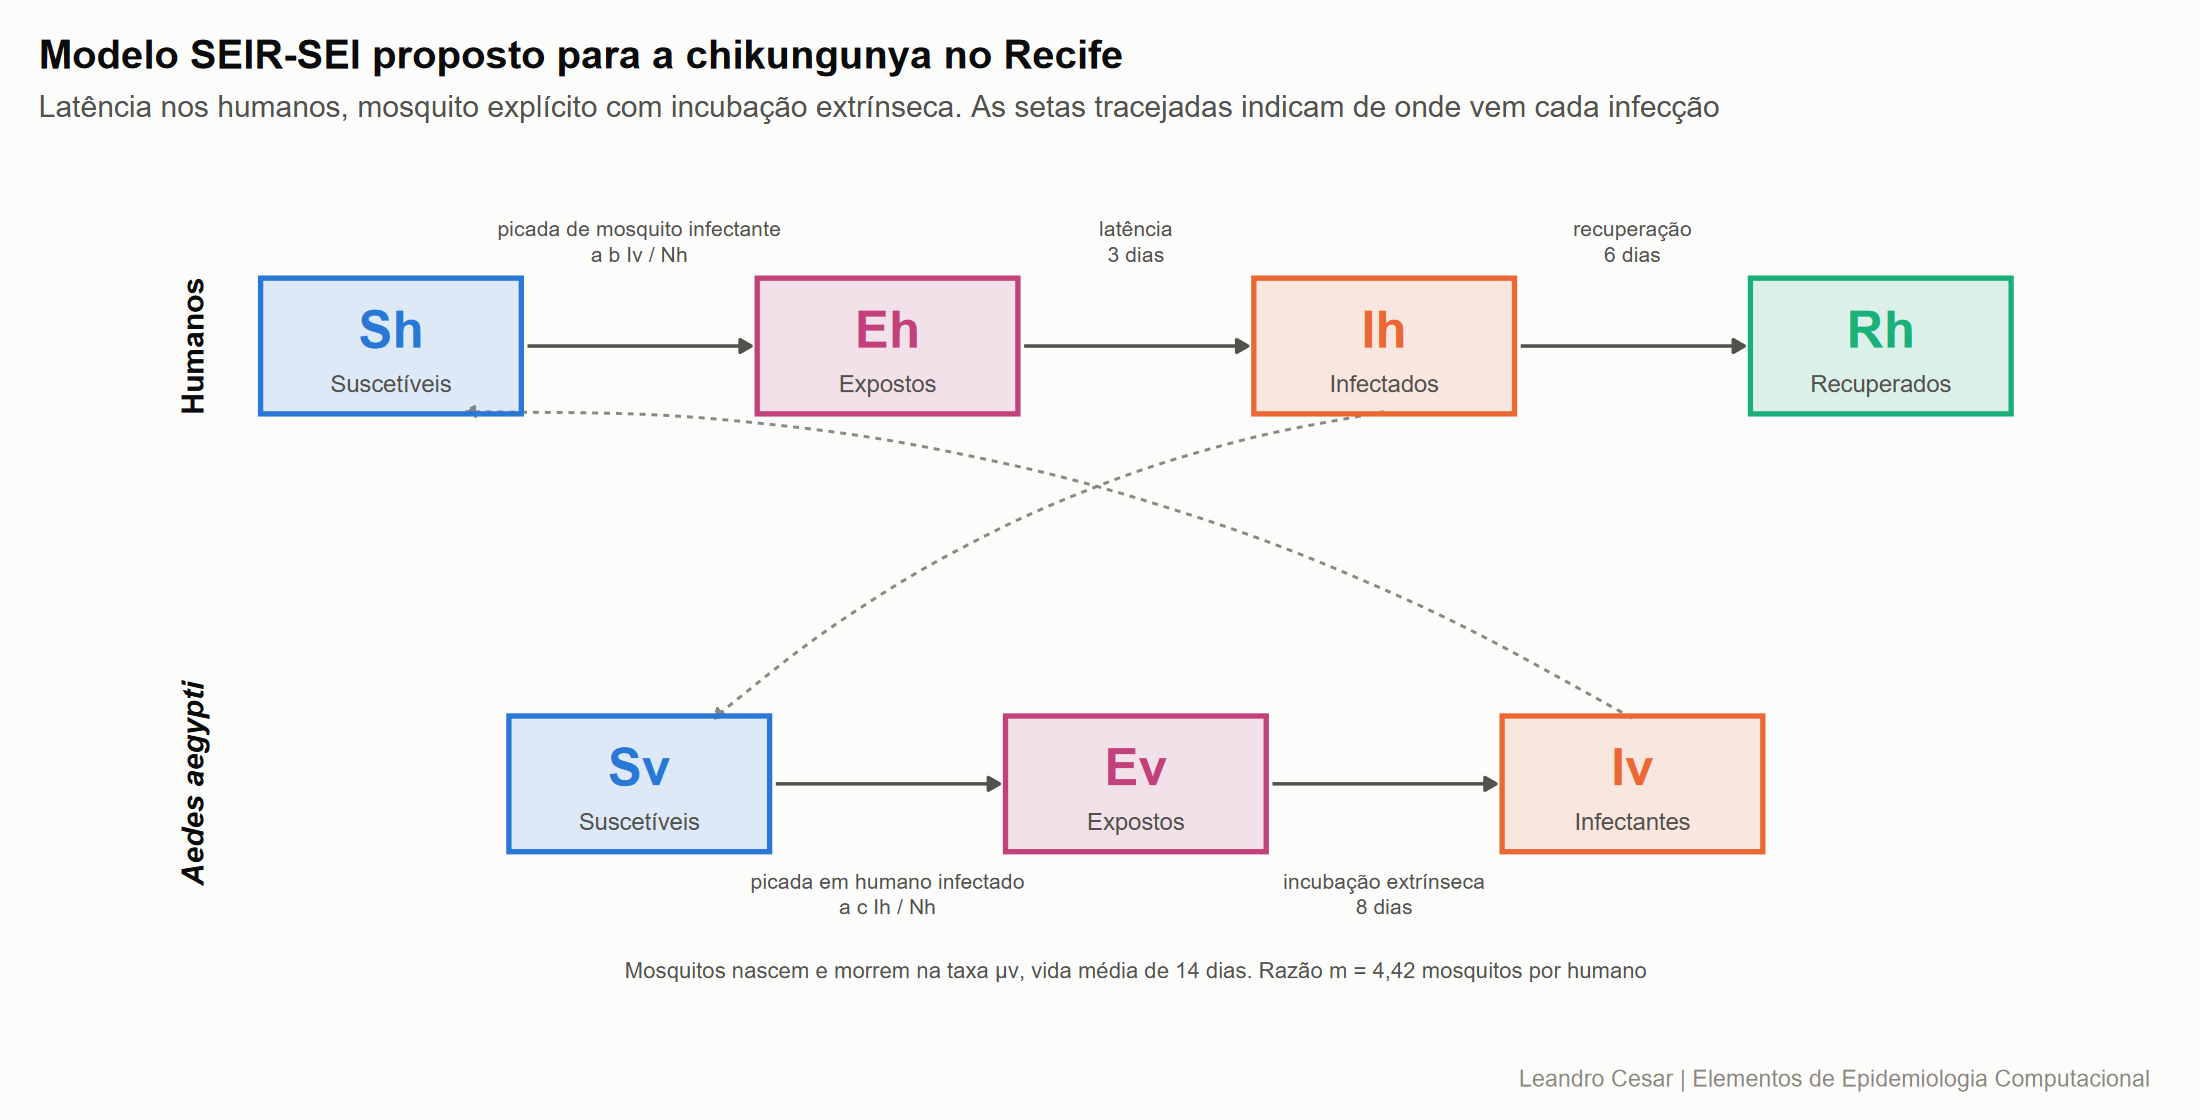
\includegraphics[width=\textwidth]{fig15_diagrama_seir_sei.png}
\caption{Estrutura do modelo SEIR-SEI com os parâmetros da Tabela \ref{tab:parametros}.}
\label{fig:diagrama}
\end{figure}

\paragraph{Parâmetros.} A Tabela \ref{tab:parametros} reúne os valores de partida. Eles vêm da compilação
de \citeonline{manore2014} para o \textit{Aedes aegypti}, com duas fontes adicionais: a latência humana
coincide com a mediana de \citeonline{rudolph2014}, e a incubação no mosquito é a média estimada por
\citeonline{christofferson2014} para a linhagem ECSA.

\begin{table}[htbp]
\centering
\caption{Parâmetros de partida do modelo SEIR-SEI.}
\label{tab:parametros}
\footnotesize
\begin{tabular}{p{5.4cm}llp{4.4cm}}
\toprule
\textbf{Parâmetro} & \textbf{Valor} & \textbf{Faixa} & \textbf{Fonte} \\
\midrule
$a$, picadas por mosquito por dia & 0,5 & 0,33 a 1 & \citeonline{manore2014} \\
$b$, infecção do mosquito para o humano & 0,24 & 0,001 a 0,35 & \citeonline{manore2014} \\
$c$, infecção do humano para o mosquito & 0,24 & 0,005 a 0,35 & \citeonline{manore2014} \\
$1/\sigma_h$, latência humana & 3 dias & 2 a 4 & \citeonline{manore2014, rudolph2014} \\
$1/\gamma$, período infeccioso humano & 6 dias & 3 a 7 & \citeonline{manore2014} \\
$1/\sigma_v$, incubação no mosquito & 8 dias & 3,8 a 14,5 & \citeonline{christofferson2014} \\
$1/\mu_v$, vida média do mosquito & 14 dias & 8 a 42 & \citeonline{manore2014} \\
$m$, mosquitos por humano & 4,42 & & escolhido para $R_{hh} = 3{,}4$ \\
\bottomrule
\end{tabular}
\end{table}

\paragraph{Números de reprodução.} Uma volta completa da transmissão tem duas metades. Um humano infectado
infecta, em média, $R_{vh} = a c m / \gamma$ mosquitos. Um mosquito recém infectado sobrevive à incubação com
probabilidade $\sigma_v/(\sigma_v + \mu_v)$ e depois pica durante $1/\mu_v$ dias, infectando
$R_{hv} = a b \sigma_v / ((\sigma_v + \mu_v)\mu_v)$ humanos. O produto $R_{hh} = R_{hv} R_{vh}$ é o número de
humanos infectados por um humano, depois de uma volta pelo mosquito. Ele corresponde ao $R_0$ de um modelo
SIR e determina o tamanho final do surto. O $R_0$ da matriz de próxima geração é $\sqrt{R_{hh}}$
\cite{manore2014}. Como a densidade de mosquitos por pessoa não é medida, $m$ foi escolhido para que
$R_{hh}$ seja 3,4, a média de \citeonline{haider2020}. Com os valores da Tabela \ref{tab:parametros},
$R_{vh} = 3{,}18$, $R_{hv} = 1{,}07$ e o $R_0$ de próxima geração é 1,84.

\paragraph{Tecnologia.} Os modelos são integrados em R 4.5.1 \cite{rcore2025} com o pacote
\texttt{deSolve} \cite{soetaert2010}. O código segue a estrutura dos cadernos do curso da disciplina e
separa modelo, integração, métricas, cenários, dados e figuras em arquivos próprios.

\subsection{Dados}

\paragraph{Notificações.} O portal de dados abertos da Prefeitura do Recife publica um arquivo por ano com
as notificações de chikungunya de 2015 a 2025 \cite{recife2026}. Apesar do nome ``casos confirmados'',
cada arquivo traz todas as notificações, com a classificação final. A série usada é a de \textbf{casos
prováveis}, a definição do Ministério da Saúde: todas as notificações de residentes no Recife, exceto as
descartadas, agregadas pela semana de início dos sintomas. Os arquivos de 2015 e 2016 trazem os códigos 1 e
2 na classificação final, que não constam no dicionário do portal. Eles foram mantidos como prováveis, e o
significado deles será confirmado com a vigilância municipal no OE2.

\paragraph{População.} Censo Demográfico 2022 do IBGE: 1.488.920 habitantes \cite{ibge2022}. As populações
por bairro e por distrito sanitário, necessárias ao OE4, também virão do Censo.

\paragraph{Sorologia.} O inquérito domiciliar de \citeonline{braga2023}, com 2.070 moradores de 5 a 65 anos
examinados entre agosto de 2018 e fevereiro de 2019, mediu IgG contra o vírus em 35,7\% (intervalo de
confiança de 95\% de 32,6\% a 38,9\%), com 22,3\%, 39,8\% e 38,6\% nos estratos alto, intermediário e baixo.

\subsection{Procedimentos por Objetivo}

\paragraph{OE1. Formular o modelo.} O sistema da Equação \ref{eq:seirsei} já está implementado. A taxa de
crescimento inicial é o maior autovalor do sistema linearizado dos compartimentos infectados no
equilíbrio sem doença, e a eficácia crítica do controle de criadouros é $1 - 1/R_{hh}$, porque $R_{hh}$ é
proporcional a $m$. O código confere a conservação das populações, a taxa de crescimento simulada contra o
autovalor e a ausência de surto com $R_{hh} < 1$.

\paragraph{OE2. Organizar os dados.} O script de download resolve os arquivos pela interface do portal,
guarda os dados brutos fora do repositório e produz a série semanal de casos prováveis para a cidade e
para cada distrito sanitário. Serão confirmados com a vigilância o significado dos códigos antigos e a
correspondência dos códigos de distrito.

\paragraph{OE3. Calibrar a primeira onda.} Os casos prováveis da semana $t$, $C_t$, serão modelados como
uma variável binomial negativa com média $\rho\, \Delta_t$, em que $\Delta_t$ é o número de humanos que
passam a infectados na semana e $\rho$ é a fração de notificação. A densidade de mosquitos vai variar ao
longo do ano, $m(t) = \bar{m}\,[1 + \delta \cos(2\pi(t - \phi)/365)]$, para representar a estação. Serão
estimados $\bar{m}$ (e portanto $R_{hh}$), $\rho$, $\delta$, $\phi$, a dispersão e a data de introdução,
por máxima verossimilhança. O inquérito entra como um segundo termo da verossimilhança: o modelo precisa
prever, para o período da coleta, a fração com anticorpos observada nos 2.070 examinados. Os intervalos
de confiança virão da verossimilhança perfilada. Séries de temperatura e chuva do INMET serão testadas
como alternativa à função cosseno.

\paragraph{OE4. Representar a heterogeneidade.} A população será dividida em grupos, por distrito sanitário
ou pelos três estratos do inquérito, cada um com sua densidade de mosquitos. A mistura entre grupos será
descrita por uma matriz com um parâmetro de acoplamento $\varepsilon$, de $\varepsilon = 0$, grupos
isolados, a $\varepsilon = 1$, mistura homogênea. O teste é se o modelo por grupos consegue reproduzir ao
mesmo tempo a série de 2015 e 2016, os 36\% do inquérito com a diferença entre estratos, e uma segunda onda
em 2021 sem supor perda de imunidade.

\paragraph{OE5. Avaliar o controle.} Com o modelo calibrado, serão simulados cenários de redução de
criadouros, que diminui o nascimento de mosquitos, e de aumento da mortalidade dos adultos, com eficácias
e datas de início diferentes, inclusive em relação à estação. O resultado de cada cenário é a taxa de
ataque, o pico e o número de casos evitados.

\paragraph{OE6. Divulgar.} O repositório reúne código, dados agregados, notebooks e o script de
conferência. Um painel vai mostrar a série observada, o ajuste do modelo e os cenários, com atualização a
cada novo arquivo anual do portal.

\subsection{Resultados Preliminares}
\label{sec:preliminares}

\subsubsection{O modelo SIR revisado}

O SIR da etapa anterior foi revisado depois da avaliação da professora (Anexo \ref{sec:anotacoes}). Com
$N = 1.488.920$, um caso inicial, período infeccioso de 6 dias \cite{manore2014} e $R_0 = 3{,}4$
\cite{haider2020}, a taxa de contágio é $\beta = R_0 \gamma = 0{,}567$ por dia. O pico acontece no dia 38,
com 438.146 suscetíveis, 515.090 infectados e 535.684 recuperados. A Tabela \ref{tab:validacao} confere a
simulação contra as três expressões analíticas do SIR. A taxa de ataque final não tem fórmula fechada e é
a raiz de $1 - a = e^{-R_0 a}$, encontrada numericamente. Simulação e raiz coincidem até a sexta casa
decimal.

\begin{table}[htbp]
\centering
\caption{Conferência do SIR contra a teoria.}
\label{tab:validacao}
\small
\begin{tabular}{lllll}
\toprule
\textbf{Grandeza} & \textbf{Expressão} & \textbf{Simulado} & \textbf{Analítico} & \textbf{Erro} \\
\midrule
Infectados no pico & $N\,(1 - (1 + \ln R_0)/R_0)$ & 515.089,7 & 515.089,5 & $4{,}5 \times 10^{-7}$ \\
Suscetíveis no pico & $N / R_0$ & 438.146,9 & 437.917,6 & $5{,}2 \times 10^{-4}$ \\
Taxa de ataque final & raiz de $1 - a = e^{-R_0 a}$ & 0,9620277 & 0,9620275 & $1{,}4 \times 10^{-7}$ \\
\bottomrule
\end{tabular}
\end{table}

Os dez cenários da Tabela \ref{tab:cenarios} cruzam as variações pedidas na atividade, taxas iguais e uma
taxa fixa com a outra variando, com os três regimes possíveis: $\beta > \gamma$, $\beta = \gamma$ e
$\gamma > \beta$.

\begin{table}[htbp]
\centering
\caption{Os dez cenários do SIR. Nos cenários sem surto, o desfecho é o total de pessoas infectadas até a
extinção.}
\label{tab:cenarios}
\footnotesize
\setlength{\tabcolsep}{4pt}
\resizebox{\textwidth}{!}{%
\begin{tabular}{clcrrrrrr}
\toprule
\textbf{N} & \textbf{Cenário} & \textbf{Regime} & $\beta$ & $\gamma$ & $R_0$ & \textbf{Pico} & \textbf{Infectados no pico} & \textbf{Desfecho} \\
\midrule
1 & Linha de base & $\beta > \gamma$ & 0,567 & 0,167 & 3,40 & dia 38 & 515.090 & 96,2\% \\
2 & Contágio 50\% maior & $\beta > \gamma$ & 0,850 & 0,167 & 5,10 & dia 23 & 720.957 & 99,4\% \\
3 & Contágio pela metade & $\beta > \gamma$ & 0,283 & 0,167 & 1,70 & dia 116 & 148.328 & 69,1\% \\
4 & Contágio igual à recuperação & $\beta = \gamma$ & 0,167 & 0,167 & 1,00 & sem surto & & 62 pessoas em 1 ano \\
5 & Contágio na metade da recuperação & $\gamma > \beta$ & 0,083 & 0,167 & 0,50 & sem surto & & 2 pessoas \\
6 & Período infeccioso dobrado & $\beta > \gamma$ & 0,567 & 0,083 & 6,80 & dia 33 & 847.936 & 99,9\% \\
7 & Recuperação igual ao contágio & $\beta = \gamma$ & 0,567 & 0,567 & 1,00 & sem surto & & 207 pessoas em 1 ano \\
8 & Recuperação acima do contágio & $\gamma > \beta$ & 0,567 & 0,708 & 0,80 & sem surto & & 5 pessoas \\
9 & Recuperação no dobro do contágio & $\gamma > \beta$ & 0,567 & 1,133 & 0,50 & sem surto & & 2 pessoas \\
10 & Mesmo $R_0$, ritmo pela metade & $\beta > \gamma$ & 0,283 & 0,083 & 3,40 & dia 76 & 515.090 & 96,2\% \\
\bottomrule
\end{tabular}}
\end{table}

Com $\gamma > \beta$, a pessoa se recupera, em média, antes de passar o vírus adiante. Enquanto quase todos
são suscetíveis, $I(t) = I_0 e^{(\beta - \gamma) t}$, que decai e vira uma reta numa escala logarítmica
(Figura \ref{fig:subcritico}). O total de infectados até a cadeia acabar é a soma $I_0(1 + R_0 + R_0^2 +
\dots) = I_0/(1 - R_0)$: 2 pessoas com $R_0 = 0{,}5$ e 5 com $R_0 = 0{,}8$, valores que a simulação reproduz.
Com $\beta = \gamma$ a prevalência fica parada e o total cresce em linha reta. Os cenários 5 e 9 têm o mesmo
$R_0$ e o mesmo total, mas o 9 se extingue mais rápido, assim como os cenários 1 e 10 têm o mesmo tamanho e
o 10 leva o dobro do tempo: a razão entre as taxas define o tamanho do surto, e a escala define a
velocidade. A Figura \ref{fig:fases} mostra a taxa de ataque para todas as combinações de $\beta$ e
$\gamma$.

\begin{figure}[htbp]
\centering
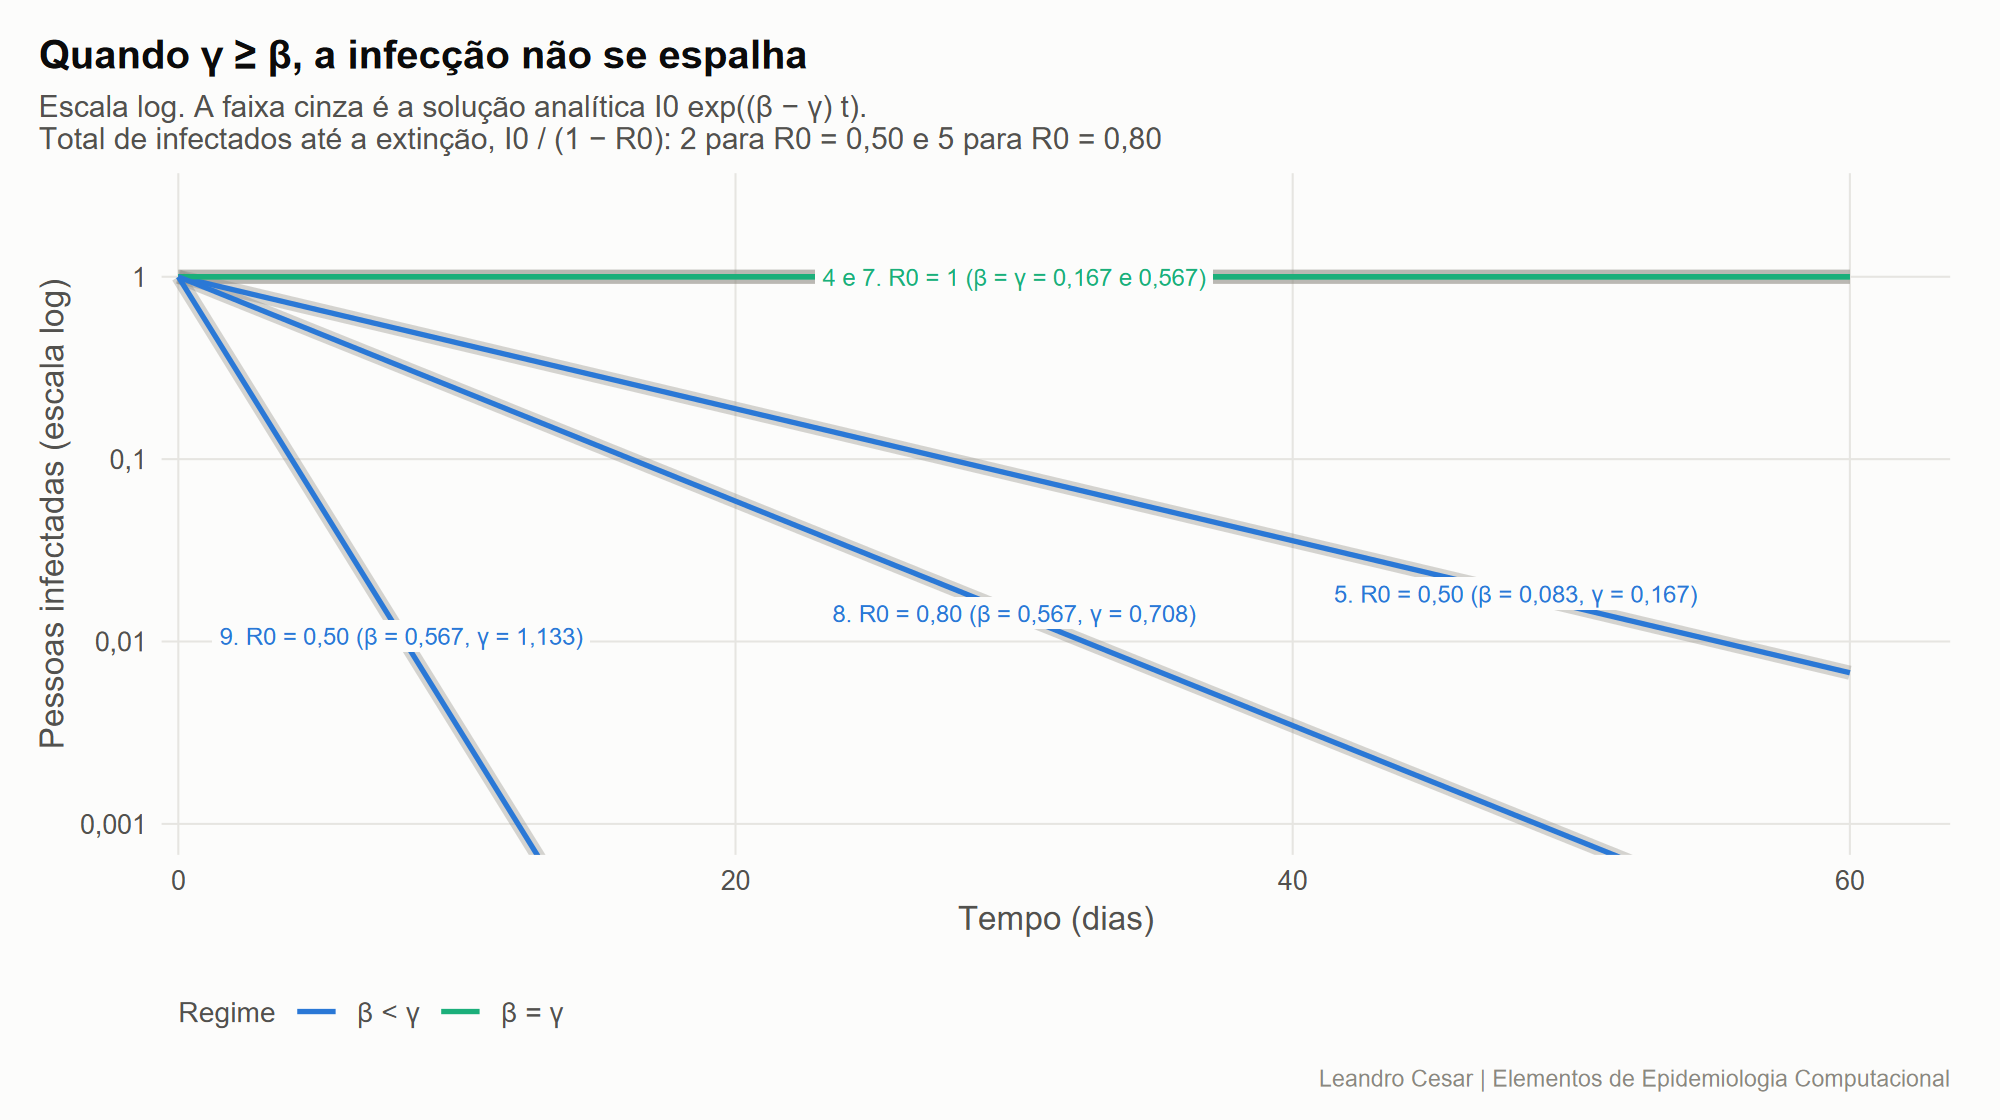
\includegraphics[width=0.92\textwidth]{fig06_regime_subcritico.png}
\caption{Cenários com $\gamma \geq \beta$ em escala logarítmica. A faixa cinza é a solução analítica.}
\label{fig:subcritico}
\end{figure}

\begin{figure}[htbp]
\centering
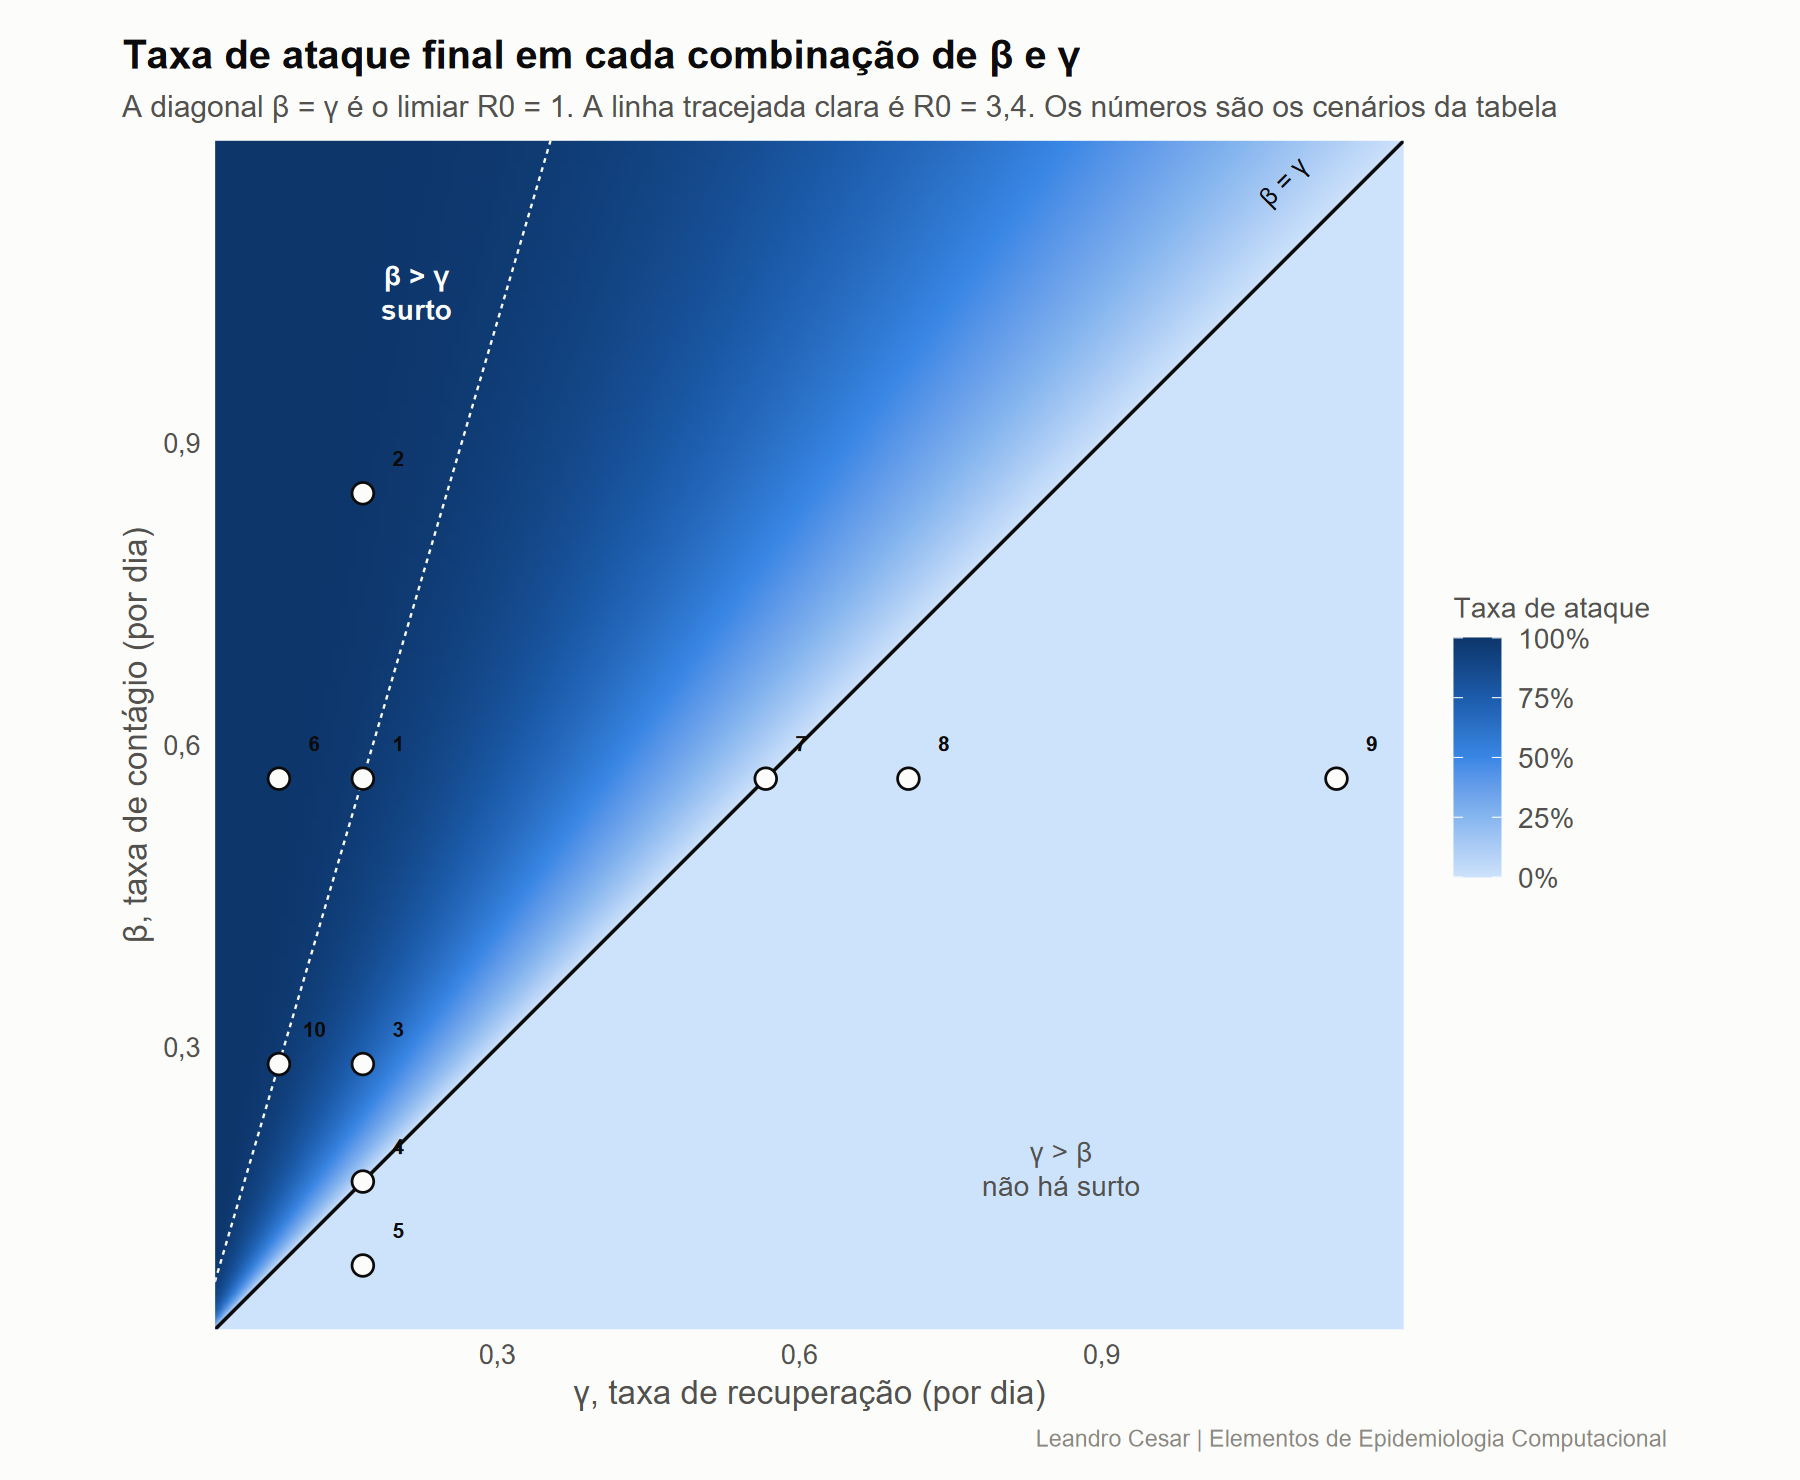
\includegraphics[width=0.8\textwidth]{fig07_mapa_fases.png}
\caption{Taxa de ataque final no plano $(\gamma, \beta)$. Abaixo da diagonal não há surto.}
\label{fig:fases}
\end{figure}

\paragraph{Controle vetorial no SIR.} Sem mosquito no modelo, o controle só pode ser uma redução de $\beta$,
o que se justifica porque a transmissão é proporcional à densidade de mosquitos \cite{smith2012}. Como não
há uma eficácia bem estabelecida para campanhas reais \cite{bowman2016}, a eficácia foi variada. Começando
no primeiro caso, o surto é evitado com redução de pelo menos $1 - 1/R_0 = 70{,}6\%$, entre 58,3\% e 76,2\%
na faixa de $R_0$ de 2,4 a 4,2. A Figura \ref{fig:inicio} varia também o dia de início. Uma redução de 80\%
evita o surto se começar no dia 0, deixa 24\% de infectados se começar no dia 30 e 84\% se começar no dia
40, logo depois do pico.

\begin{figure}[htbp]
\centering
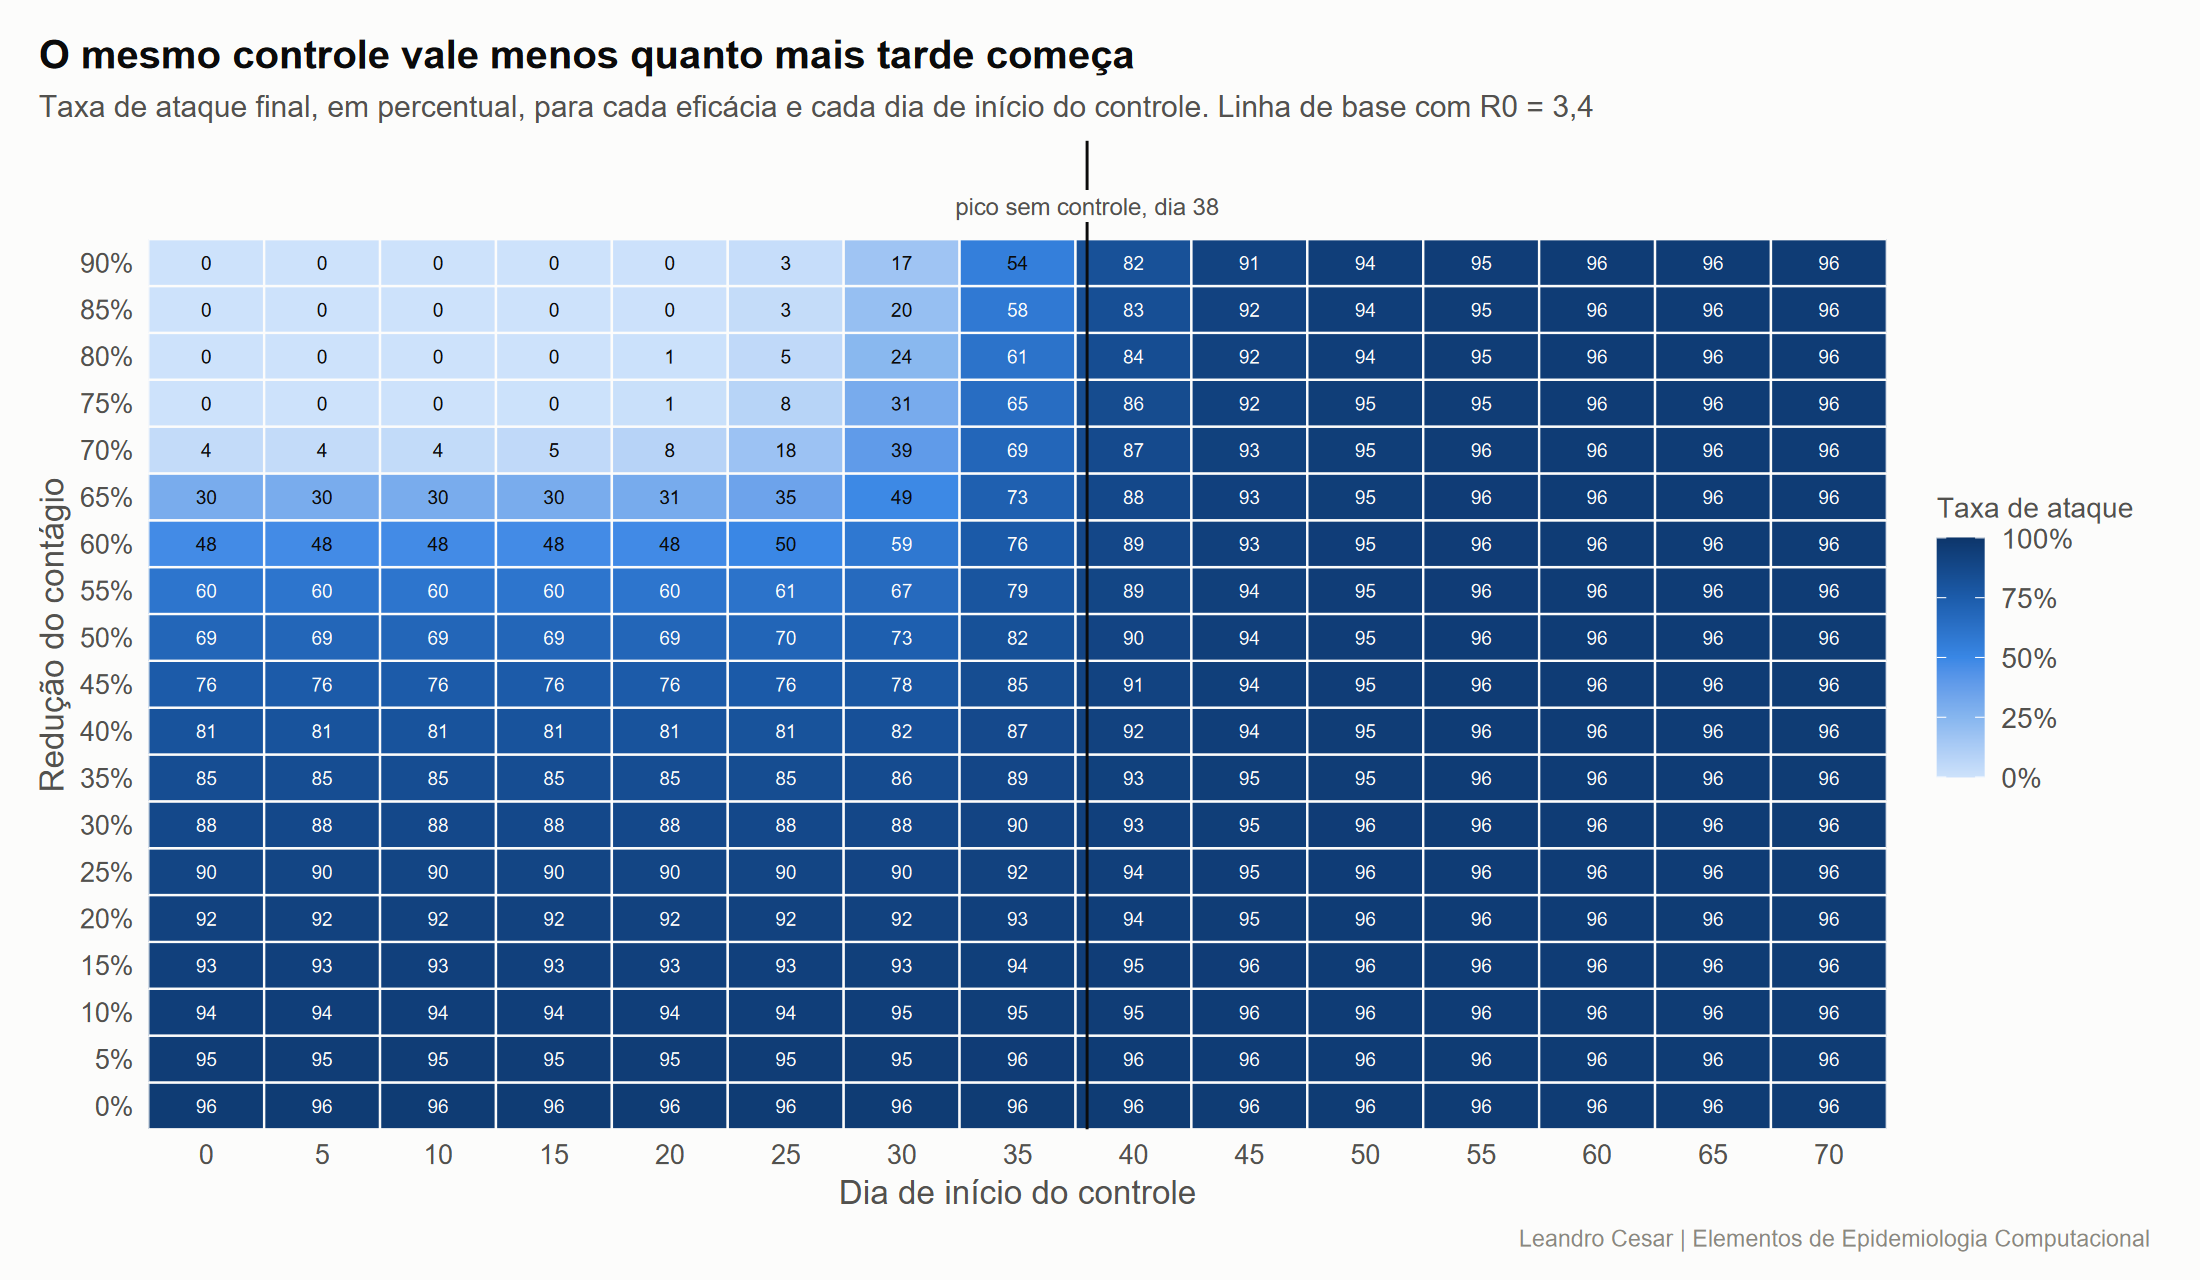
\includegraphics[width=0.95\textwidth]{fig10_controle_inicio.png}
\caption{Taxa de ataque final, em percentual, por eficácia e dia de início do controle no SIR.}
\label{fig:inicio}
\end{figure}

\paragraph{Reinfecção.} Para testar a hipótese de imunidade permanente, o SIR foi estendido com uma taxa de
perda de imunidade. Se a imunidade durasse em média 10 anos, uma segunda onda viria cerca de 6,7 anos
depois da primeira. Se durasse 2 anos, a doença ficaria endêmica, com cerca de 8.600 infectados a qualquer
momento. Nenhum dos dois quadros é necessário para explicar os dados do Recife, como mostra a discussão
abaixo, e a evidência imunológica sustenta a imunidade duradoura \cite{nitatpattana2014,
srikiatkhachorn2016, auerswald2018}.

\subsubsection{Os dados do Recife}

A Figura \ref{fig:dados} mostra a série de casos prováveis. A primeira onda começa em agosto de 2015 e tem
pico na semana de 14 de fevereiro de 2016, com 683 casos. A segunda, em 2021, chega a 1.319 casos na
semana de 30 de maio.

\begin{figure}[htbp]
\centering
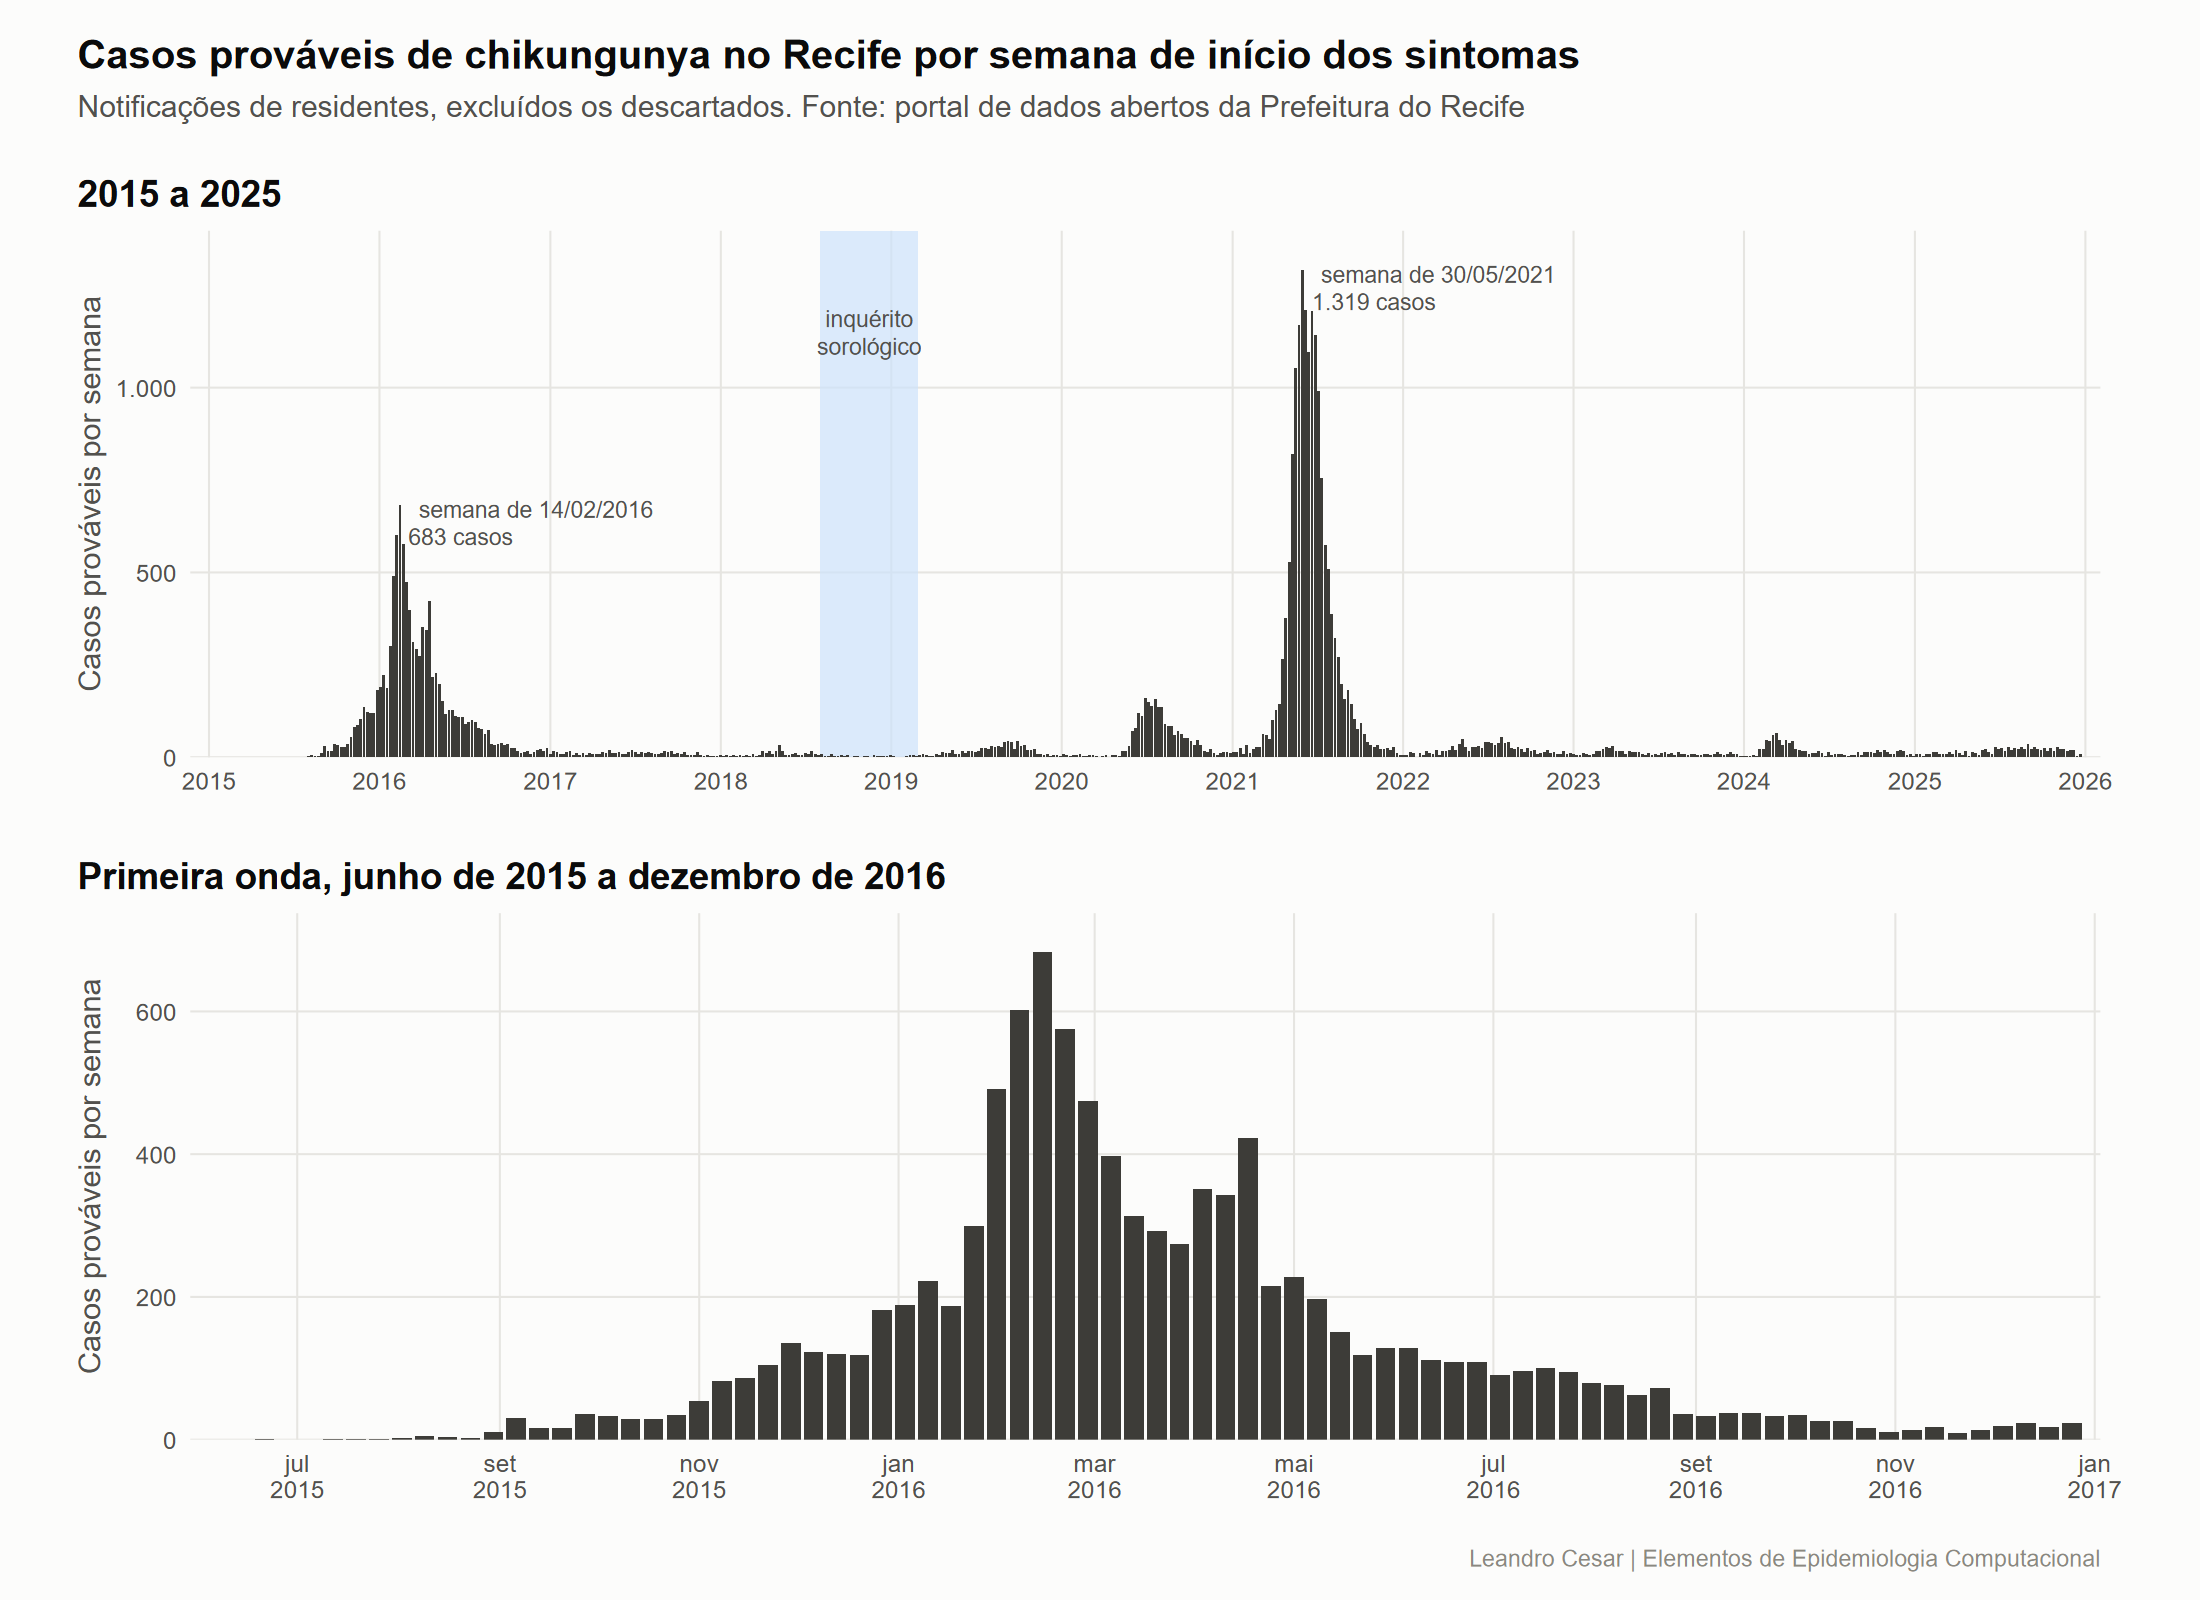
\includegraphics[width=\textwidth]{fig12_dados_recife.png}
\caption{Casos prováveis de chikungunya no Recife por semana de início dos sintomas.}
\label{fig:dados}
\end{figure}

Na fase de crescimento da primeira onda, de 30 de agosto de 2015 a 31 de janeiro de 2016, os casos
cresceram à taxa $r = 0{,}0208$ por dia (intervalo de confiança de 95\% de 0,0183 a 0,0232), dobrando a cada
33 dias (Figura \ref{fig:crescimento}). Cada modelo precisa de um número de reprodução diferente para
crescer nesse ritmo, porque cada um tem um intervalo de geração, o tempo entre uma infecção e a seguinte
na cadeia, diferente. No SIR, $r = \gamma(R_0 - 1)$ e portanto $R_0 = 1{,}12$. No SEIR-SEI, em que a geração
inclui a latência humana, a incubação no mosquito e a vida do mosquito, o valor exigido é $R_{hh} = 1{,}71$.
A Tabela \ref{tab:estimativas} reúne essas estimativas com a da literatura e a do inquérito.

\begin{figure}[htbp]
\centering
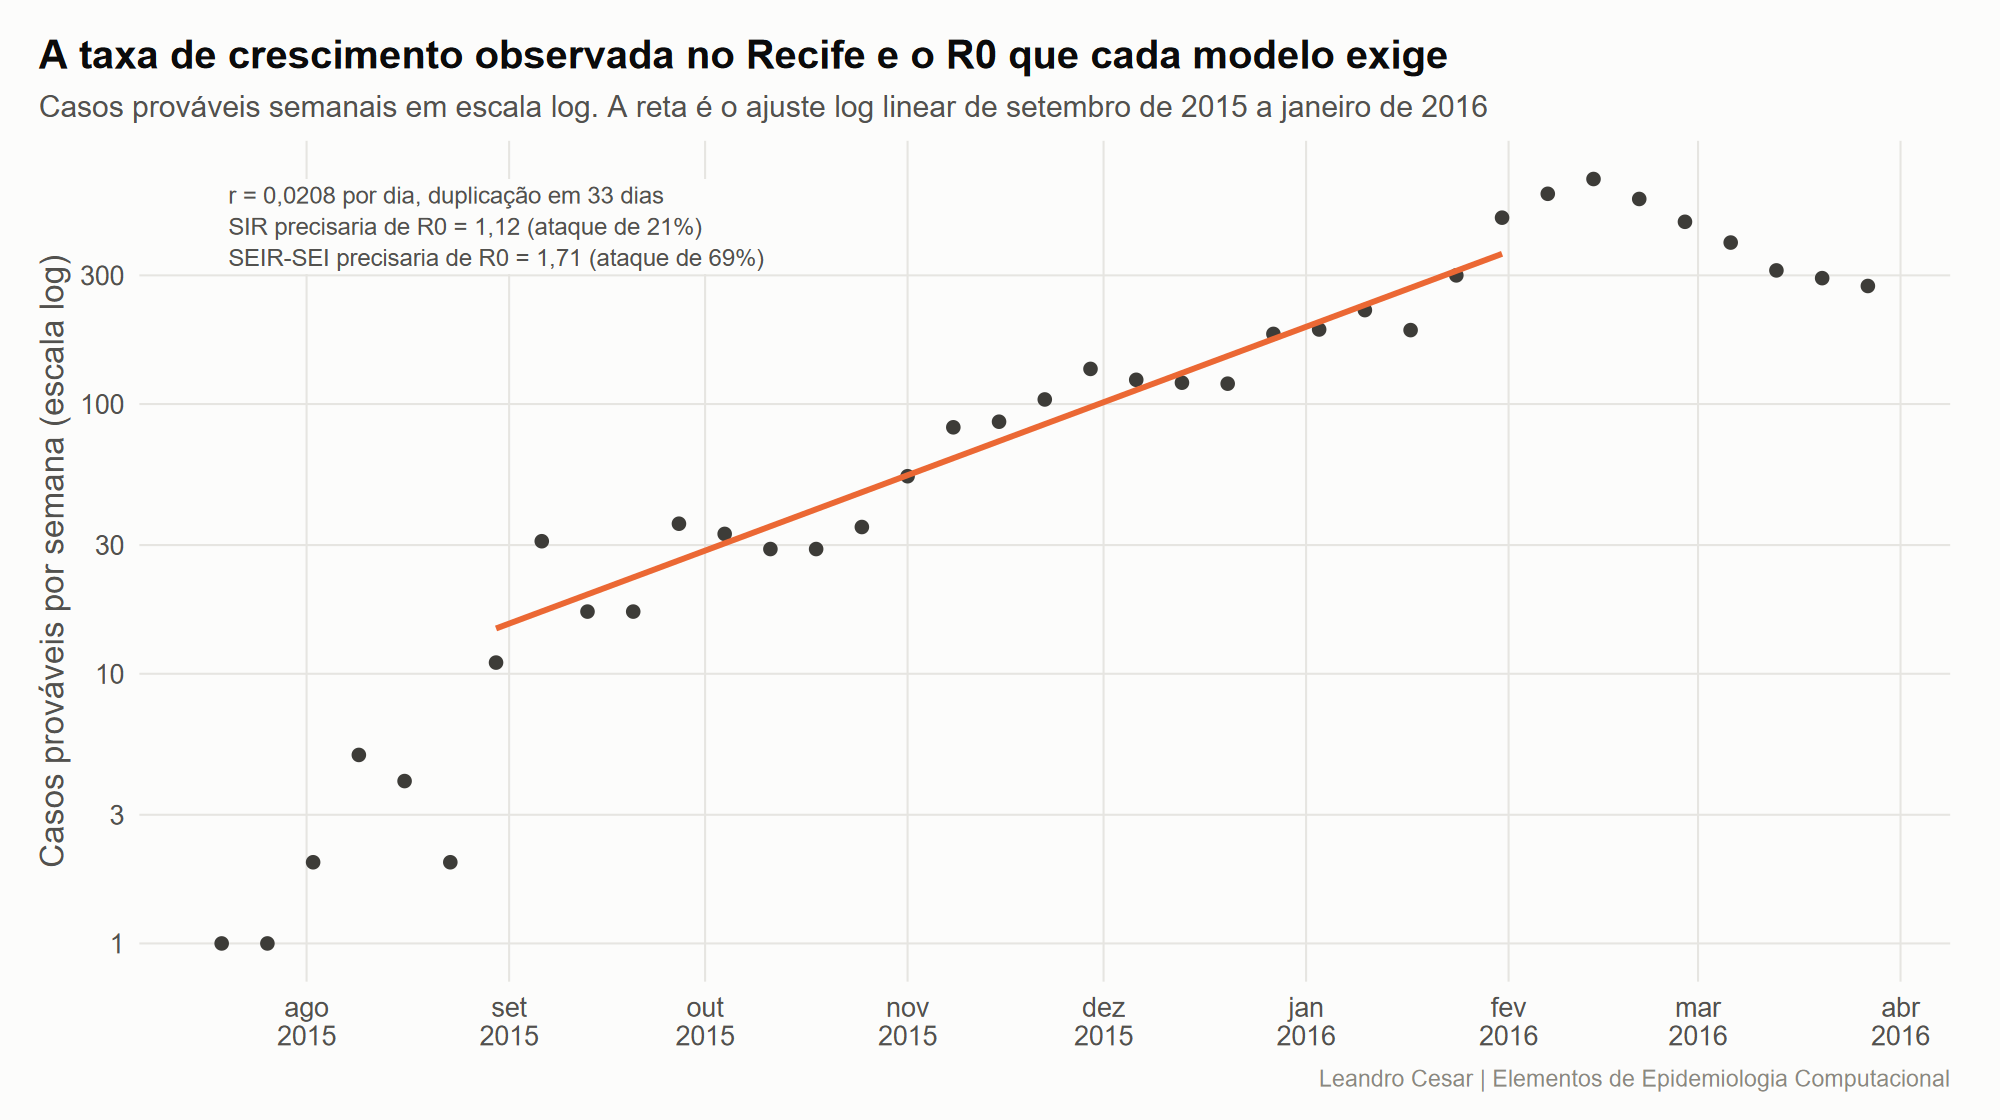
\includegraphics[width=0.92\textwidth]{fig13_crescimento_observado.png}
\caption{Taxa de crescimento da primeira onda, em escala logarítmica, e o $R_0$ que cada modelo exige.}
\label{fig:crescimento}
\end{figure}

\begin{table}[htbp]
\centering
\caption{Estimativas do número de reprodução de humano para humano e a taxa de ataque que cada uma implica
sob mistura homogênea.}
\label{tab:estimativas}
\small
\begin{tabular}{lcc}
\toprule
\textbf{Origem} & \textbf{$R_{hh}$} & \textbf{Taxa de ataque} \\
\midrule
Literatura \cite{haider2020} & 3,40 & 96\% \\
Crescimento observado, lido pelo SEIR-SEI & 1,71 & 69\% \\
Inquérito sorológico \cite{braga2023} & 1,24 & 36\% \\
Crescimento observado, lido pelo SIR & 1,12 & 21\% \\
\bottomrule
\end{tabular}
\end{table}

\subsubsection{O modelo SEIR-SEI}

Com o mesmo $R_{hh} = 3{,}4$, o SEIR-SEI cresce a 0,053 por dia, contra 0,40 do SIR, e o pico passa do dia 38
para o dia 271, com 115.189 infectados em vez de 515.090 (Figura \ref{fig:comparacao}). A taxa de ataque
quase não muda, 94,9\% contra 96,2\%, porque o tamanho final depende de $R_{hh}$. A ordem de grandeza do
tempo até o pico fica próxima da observada no Recife, cerca de seis meses, que o SIR erra por um fator de
cerca de cinco. A taxa de crescimento simulada, 0,0534 por dia, coincide com o autovalor do sistema
linearizado, 0,0533 por dia.

\begin{figure}[htbp]
\centering
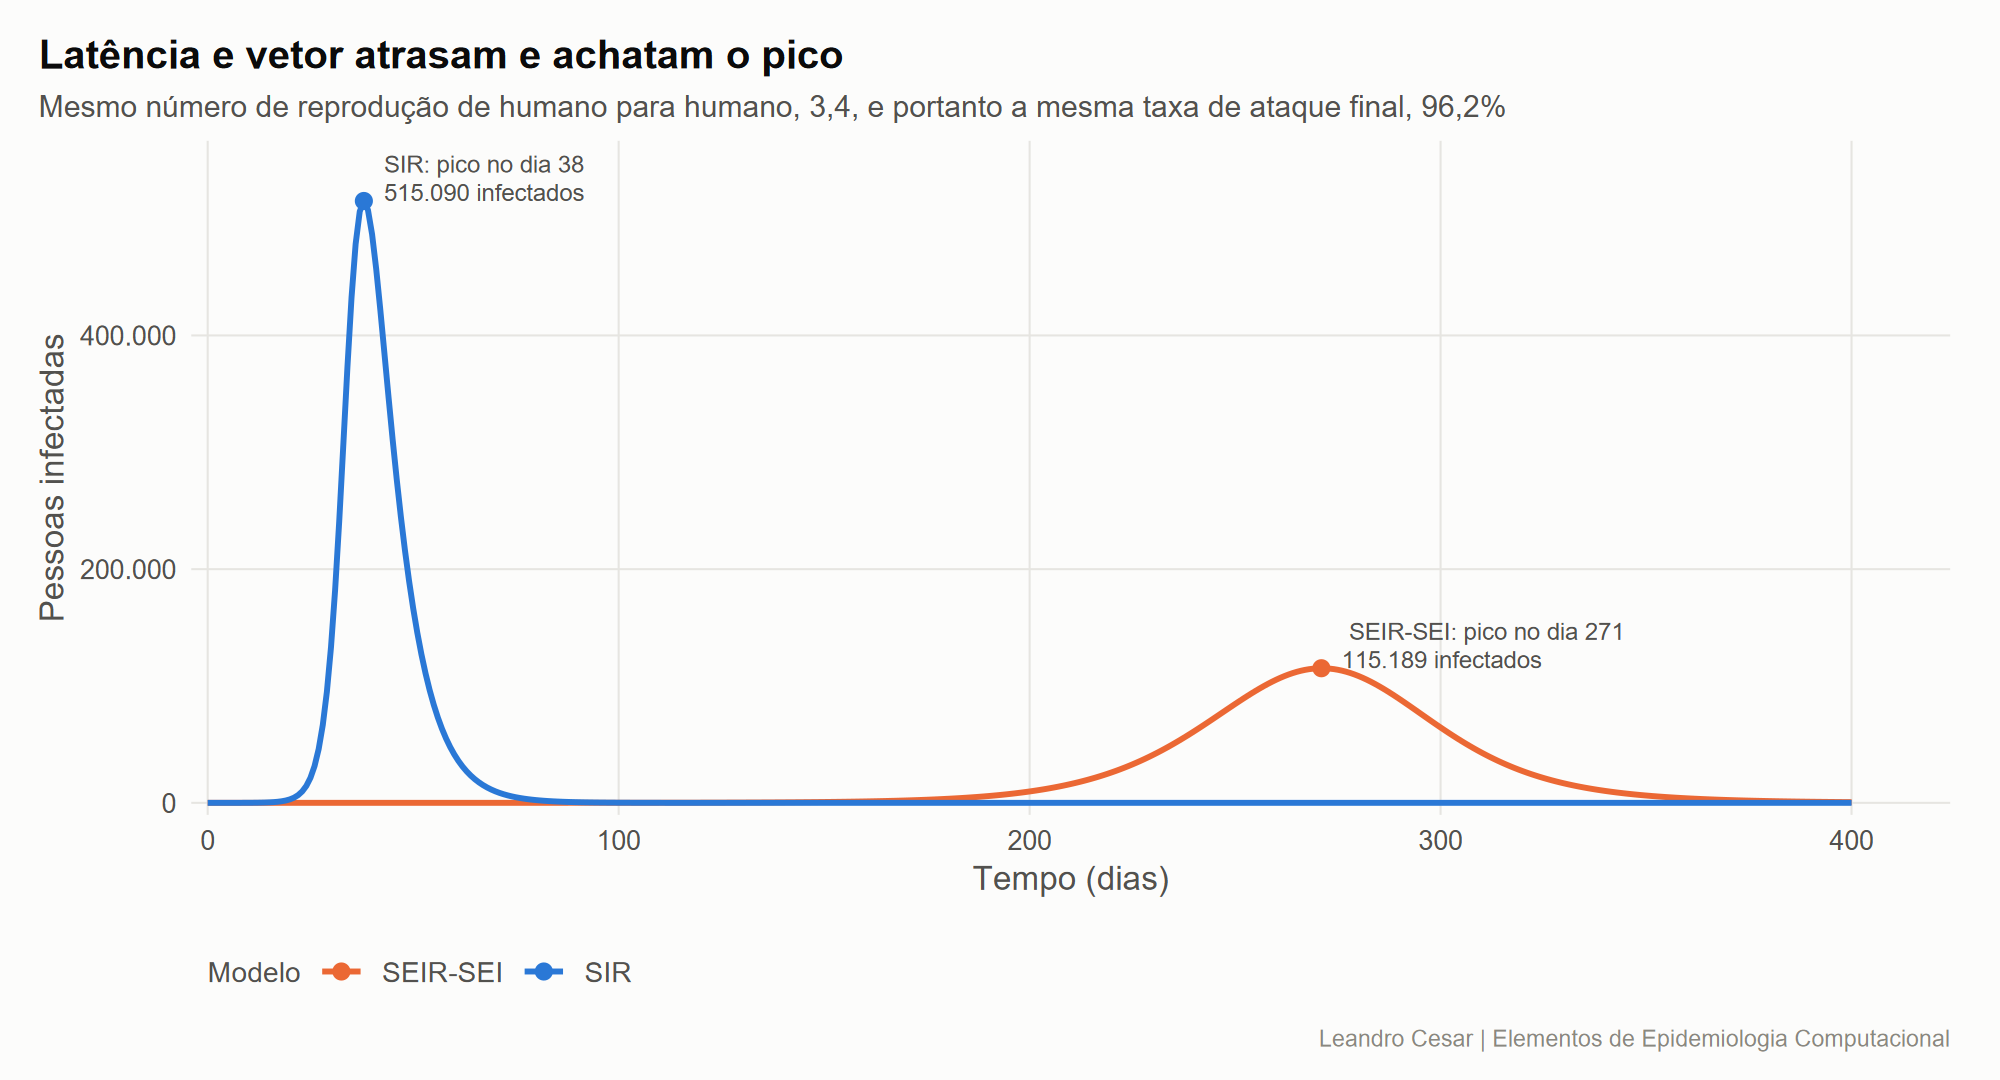
\includegraphics[width=0.92\textwidth]{fig16_sir_vs_seir_sei.png}
\caption{SIR e SEIR-SEI com o mesmo número de reprodução de humano para humano.}
\label{fig:comparacao}
\end{figure}

No SEIR-SEI, o controle de criadouros reduz o nascimento de mosquitos, e a população adulta só diminui à
medida que os mosquitos existentes morrem (Figura \ref{fig:controle}). Com redução de 80\%, os infectados
ainda crescem nas duas semanas seguintes ao início, e a taxa de ataque fica em 0,6\%, 25\% ou 76\% conforme
o controle comece no dia 120, 200 ou 250. A eficácia crítica é a mesma do SIR, $1 - 1/3{,}4 = 70{,}6\%$.
Quem usasse o $R_0$ de próxima geração, 1,84, calcularia $1 - 1/1{,}84 = 46\%$ e subestimaria o esforço
necessário, o que mostra por que a definição de $R_0$ precisa ser explícita.

\begin{figure}[htbp]
\centering
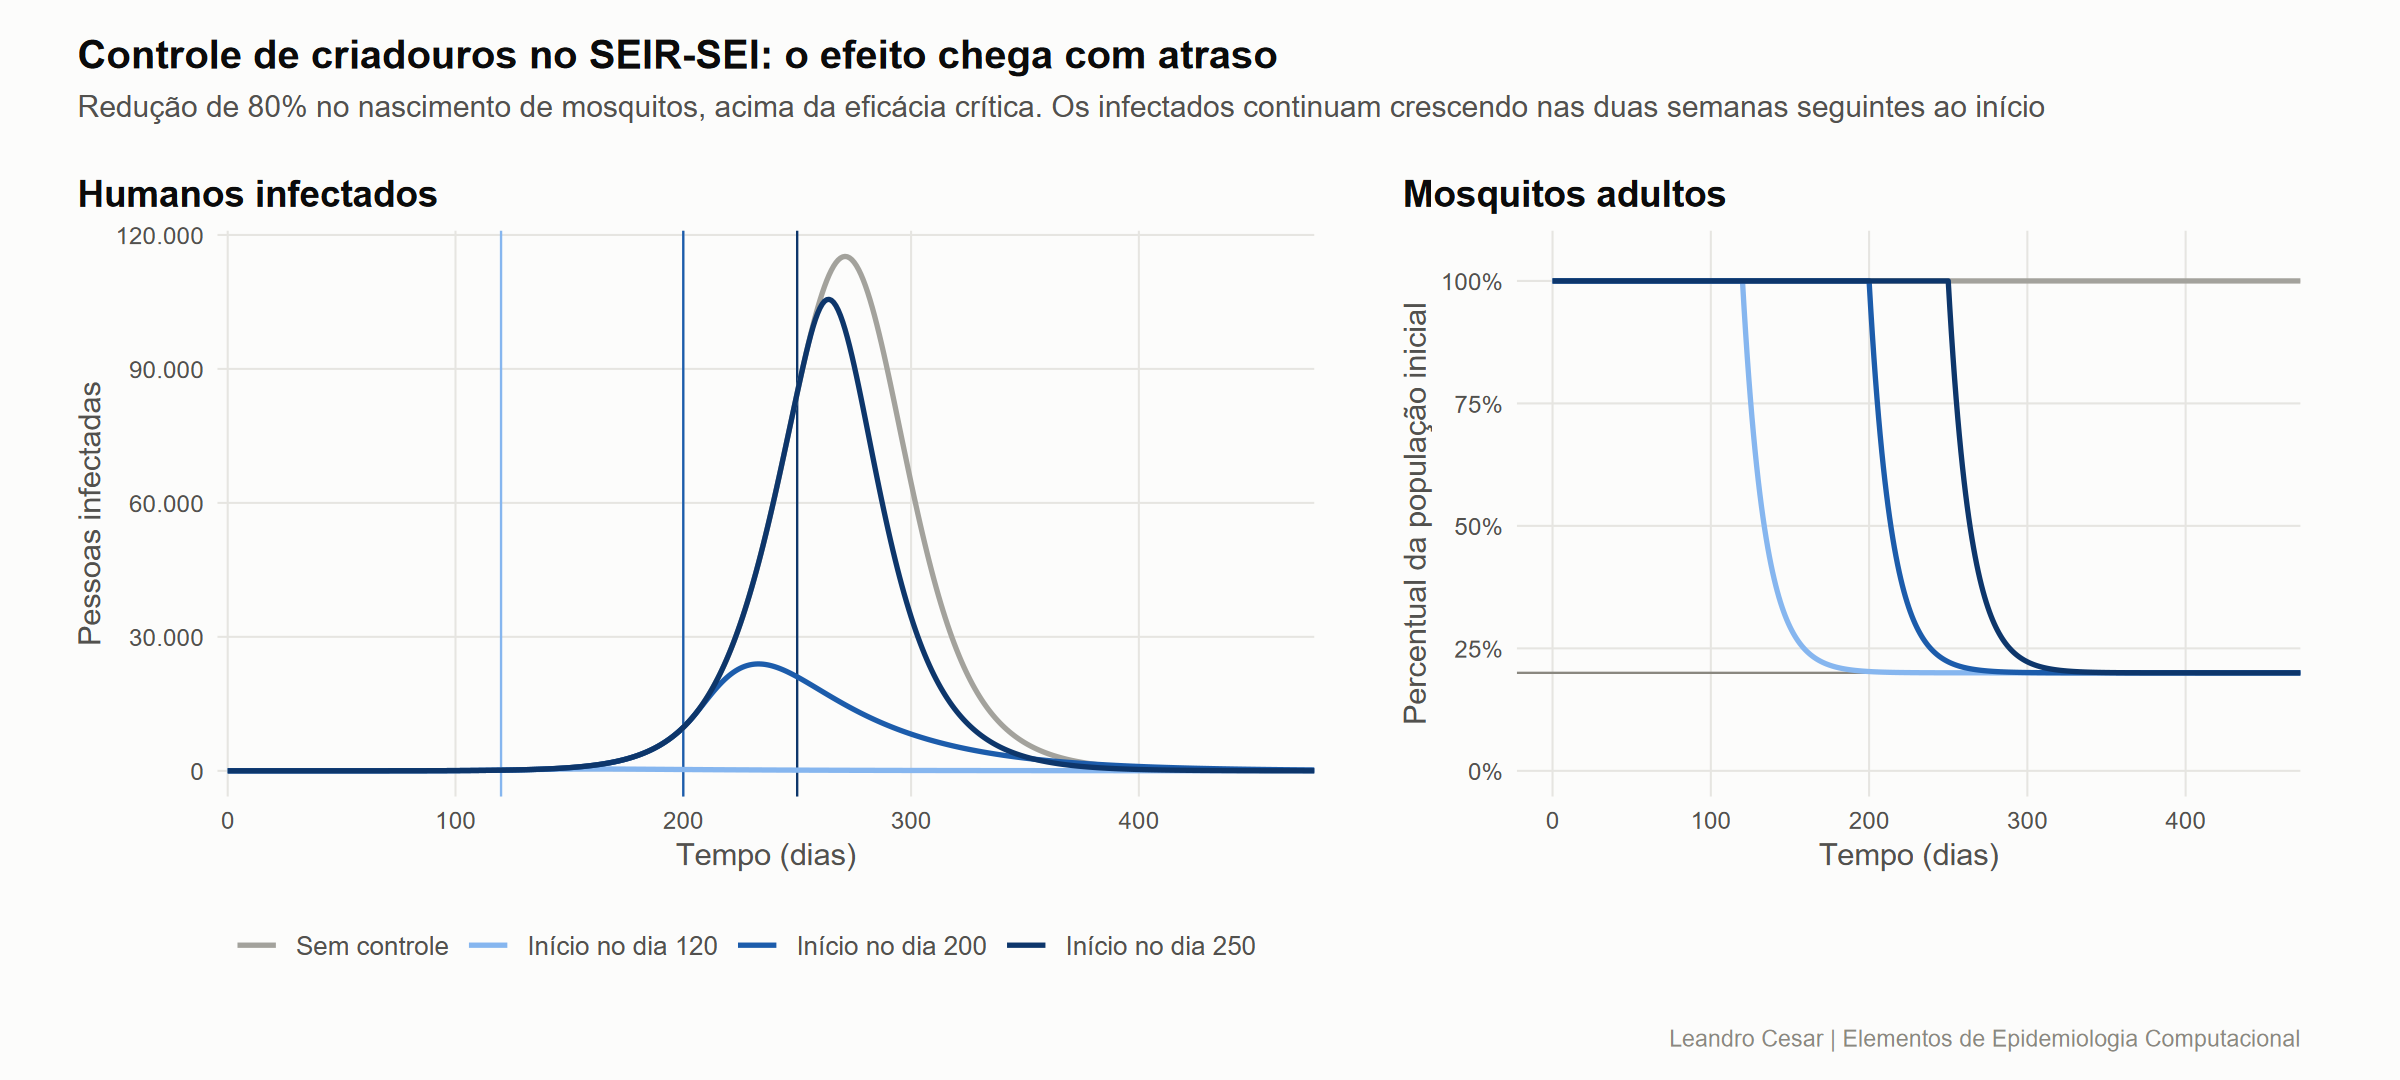
\includegraphics[width=\textwidth]{fig17_controle_vetorial.png}
\caption{Controle de criadouros no SEIR-SEI, iniciado em três momentos da fase de crescimento.}
\label{fig:controle}
\end{figure}

\subsubsection{Discussão dos resultados preliminares}

Os dados do Recife medem as distâncias entre os modelos homogêneos e a epidemia real em três frentes.

\textbf{Tamanho.} Com o $R_0$ da literatura, o SIR prevê que 96,2\% da população se infecte, e o inquérito
encontrou 35,7\% (Figura \ref{fig:sorologia}). Resolvendo a equação do tamanho final para $R_0$, os 35,7\%
correspondem a $R_0 = -\ln(1 - a)/a = 1{,}24$ sob mistura homogênea. A diferença entre o estrato alto,
22,3\%, e os demais, perto de 39\%, mostra que a cidade não se infectou por igual. Isso pesa contra a
mistura homogênea e é o que o OE4 vai testar.

\begin{figure}[htbp]
\centering
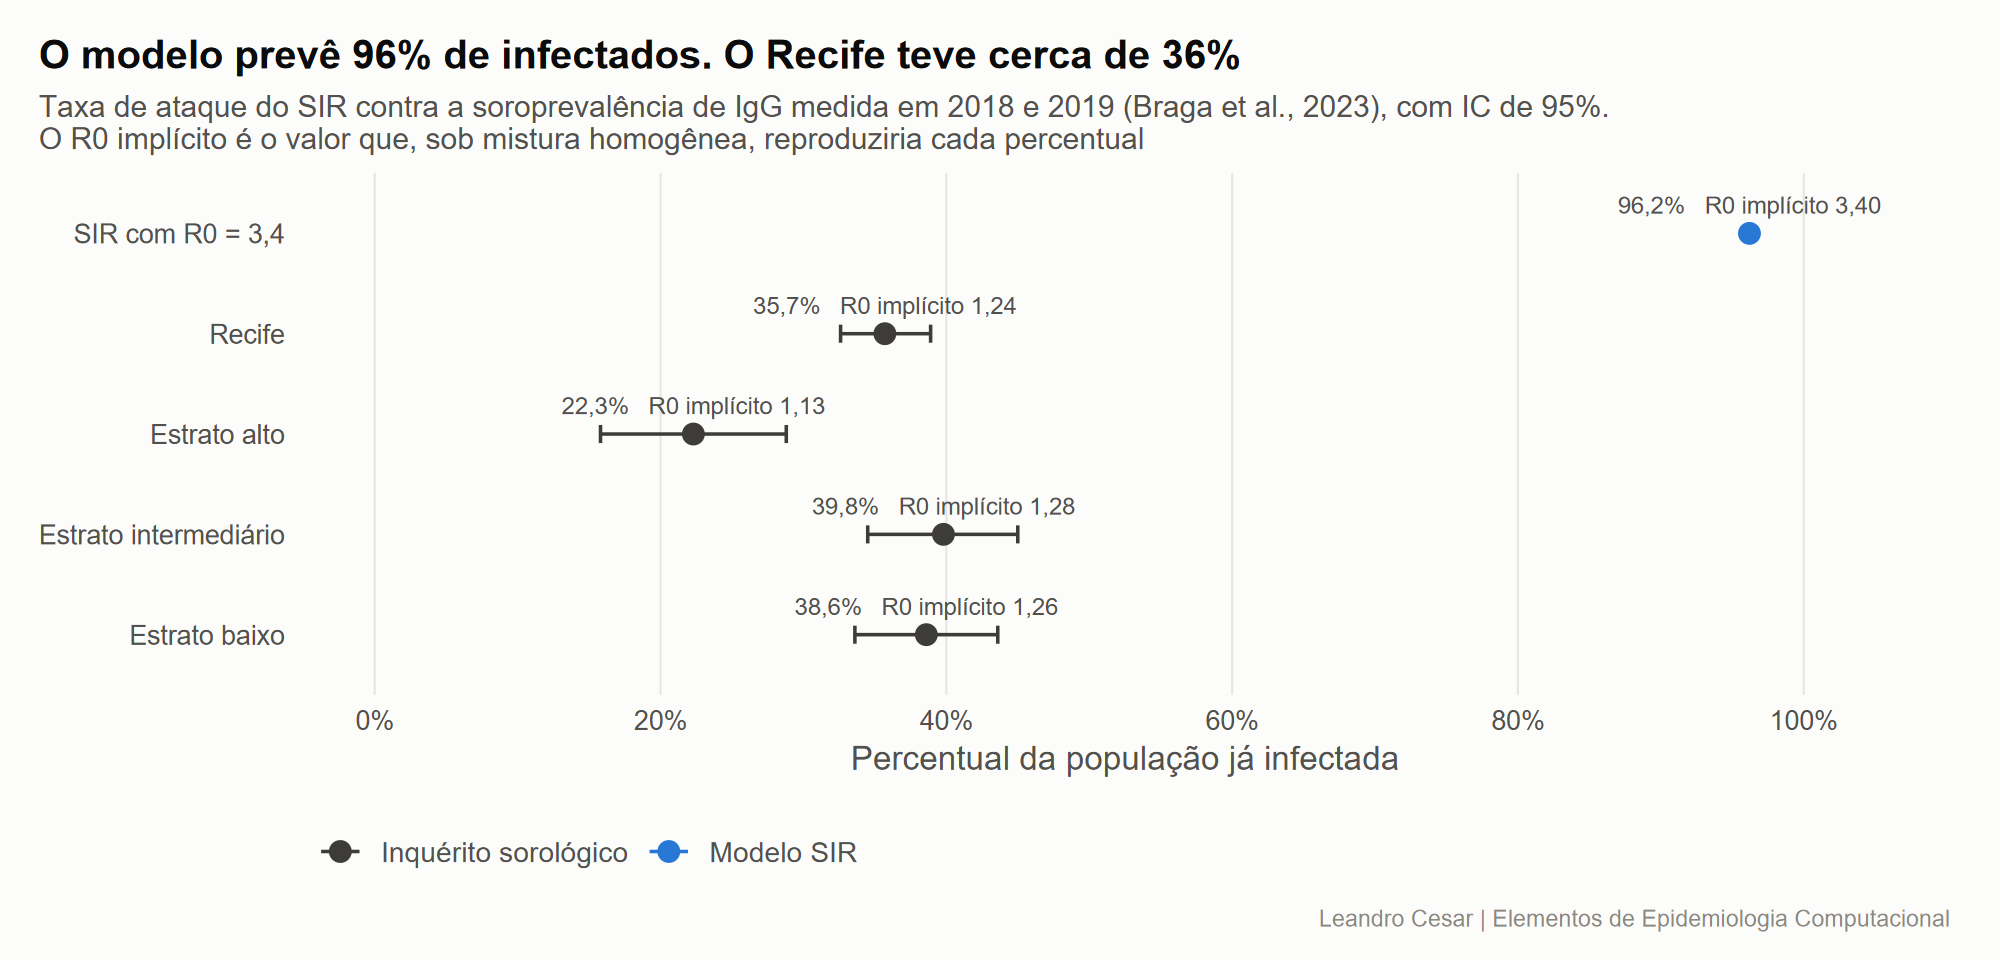
\includegraphics[width=0.92\textwidth]{fig14_sorologia.png}
\caption{Taxa de ataque do SIR contra a soroprevalência medida no Recife, com o $R_0$ implícito.}
\label{fig:sorologia}
\end{figure}

\textbf{Ritmo.} O SIR põe o pico 38 dias depois do primeiro caso, e a primeira onda levou cerca de seis
meses entre o início do crescimento e o pico. O SEIR-SEI corrige a ordem de grandeza, o que confirma a
sugestão de incluir o vetor e a latência. Como mostra a Tabela \ref{tab:estimativas}, a mesma série
observada implica números de reprodução diferentes em cada modelo: a estrutura do modelo não é um detalhe,
ela muda o que se conclui dos dados.

\textbf{Notificação.} Foram 9.989 casos prováveis em 2015 e 2016, 0,7\% da população. Se 35,7\% se
infectaram, foram cerca de 531 mil infecções, ou 53 para cada caso provável. \citeonline{braga2023} chegam a
uma razão parecida, de cerca de 45, com outra contagem de notificações. A fração de notificação, portanto,
precisa ser estimada junto com a transmissão, como prevê o OE3.

\textbf{Reinfecção ou heterogeneidade.} A onda de 2021 poderia sugerir perda de imunidade. Mas o inquérito,
feito antes dela, mostra que cerca de 64\% da população nunca tinha sido infectada, o que basta para uma nova
onda sem reinfecção. A hipótese mais simples é que a primeira onda parou antes de atingir toda a cidade,
por causa da estação e da distribuição desigual da transmissão entre os grupos.

Nenhum modelo homogêneo reproduz ao mesmo tempo a velocidade e o tamanho da primeira onda: o SEIR-SEI,
ajustado pelo crescimento, ainda prevê 69\% de infectados. A diferença que sobra é o objeto da proposta. Há
também limitações nos dados que o projeto precisa enfrentar: o significado dos códigos antigos de
classificação, e o fato de que parte do crescimento inicial das notificações pode refletir a atenção
crescente dos serviços a uma doença nova, e não só a transmissão.

\subsection{Aspectos éticos}

A pesquisa é computacional e usa apenas dados secundários: as notificações publicadas no portal de dados
abertos da Prefeitura do Recife \cite{recife2026}, a população do Censo 2022 e os resultados agregados
publicados do inquérito sorológico. Não há contato com participantes. Os arquivos do portal são públicos,
mas trazem campos que permitem identificar pessoas, como endereço e data de nascimento. Por isso esses
arquivos são guardados apenas localmente, fora do repositório, e o projeto usa e publica somente contagens
agregadas por semana e por distrito, sem possibilidade de identificação individual. A Resolução CNS
510/2016 dispensa de registro no sistema CEP/CONEP a pesquisa com informações de acesso público e a
pesquisa com bancos de dados de informações agregadas \cite{cns510}. Como o tratamento parte de registros
individuais, antes da execução a dispensa será confirmada com o Comitê de Ética em Pesquisa da UFRPE,
considerando também a Resolução CNS 738/2024, que trata do uso de bancos de dados em pesquisa
\cite{cns738}.

\section{Cronograma}
\label{sec:cronograma}

O projeto está planejado para seis meses. A Tabela \ref{tab:cronograma} relaciona cada etapa ao objetivo
específico correspondente.

\begin{table}[h]
\centering
\small
\begin{tabular}{|p{5.9cm}|c|c|c|c|c|c|}
\hline
\textbf{Atividades} & \textbf{Mês 1} & \textbf{Mês 2} & \textbf{Mês 3} & \textbf{Mês 4} & \textbf{Mês 5} & \textbf{Mês 6} \\ \hline
1. Revisão bibliográfica e formulação do modelo (OE1) & X & X & & & & \\ \hline
2. Organização dos dados por distrito (OE2) & X & X & & & & \\ \hline
3. Calibração da primeira onda (OE3) & & X & X & X & & \\ \hline
4. Modelo por grupos e onda de 2021 (OE4) & & & X & X & X & \\ \hline
5. Cenários de controle vetorial (OE5) & & & & X & X & \\ \hline
6. Relatório, repositório e painel (OE6) & & & & & X & X \\ \hline
\end{tabular}
\caption{Cronograma de execução do projeto.}
\label{tab:cronograma}
\end{table}

\section{Resultados Esperados}
\label{sec:resultados_esperados}

\begin{itemize}

  \item \textbf{Modelo calibrado.} Um modelo SEIR-SEI ajustado à primeira onda de chikungunya no Recife,
  com estimativas e intervalos de confiança para o número de reprodução, a fração de notificação e a
  sazonalidade do vetor.

  \item \textbf{Imunidade remanescente.} Estimativas da fração da população ainda suscetível na cidade e,
  com o modelo por grupos, em cada distrito sanitário ou estrato.

  \item \textbf{Cenários de controle.} Comparação entre redução de criadouros e aumento da mortalidade dos
  mosquitos adultos, com diferentes eficácias e momentos de início, expressa em casos evitados.

  \item \textbf{Implementação computacional aberta.} Repositório público com código, dados agregados,
  notebooks e o script que regenera todos os resultados conferindo-os contra a teoria.

  \item \textbf{Painel de monitoramento.} Um painel que mostra a série observada, o ajuste do modelo e os
  cenários, atualizado a cada novo arquivo anual do portal de dados abertos.

  \item \textbf{Impacto institucional.} Um relatório técnico que possa ser apresentado à vigilância
  epidemiológica do Recife, e material didático para a disciplina de Epidemiologia Computacional, que
  mostra o caminho do SIR ao modelo com vetor usando dados da própria cidade.

\end{itemize}

\section{Declaração de uso de inteligência artificial}
\label{sec:uso_ia}

Este trabalho usou o assistente de programação Claude Code, com o modelo de linguagem Claude Opus 5.5, da
empresa Anthropic \cite{anthropic2026}. O uso está identificado a seguir.

\begin{itemize}
  \item \textbf{Código.} Escrita e revisão do código em R dos modelos, dos cenários, do tratamento dos dados
  e das figuras, e do script que confere os resultados contra as expressões analíticas.
  \item \textbf{Referências.} Busca de literatura e conferência das referências nas fontes primárias. Nessa
  conferência foi encontrada e corrigida uma citação errada da versão anterior do trabalho, que atribuía o
  $R_0$ de 3,4 a outros autores.
  \item \textbf{Texto.} Complementação e ajuste da redação a partir do texto base elaborado pelo autor, bem
  como revisão dos trechos deste documento e dos notebooks do repositório.
\end{itemize}

Os resultados numéricos não foram gerados pela ferramenta: todos vêm do código do repositório, que os
confere contra as expressões analíticas sempre que as figuras são regeneradas. A exploração da estrutura
dos arquivos do portal de dados abertos, as decisões de modelagem, a escolha dos parâmetros e a
interpretação dos resultados foram realizadas pelo autor, que conferiu as referências citadas e é
responsável por todo o conteúdo.

\newpage
\renewcommand{\refname}{{Referências bibliográficas}}
\bibliographystyle{abntex2-alf}
\bibliography{referencias}


% para incluir anexos
\appendix
\section{Anexo: respostas às anotações da etapa anterior}
\label{sec:anotacoes}

A versão anterior deste estudo, entregue como atividade do Módulo I, recebeu cinco anotações da
professora. A Tabela \ref{tab:anotacoes} indica onde cada uma foi respondida nos resultados preliminares.

\begin{table}[htb]
\centering
\caption{Anotações da avaliação do Módulo I e onde foram respondidas.}
\label{tab:anotacoes}
\small
\begin{tabular}{p{5.2cm}p{9.6cm}}
\toprule
\textbf{Anotação} & \textbf{Resposta} \\
\midrule
``Onde está essa discussão?'', sobre o confronto entre a taxa de ataque e a soroprevalência &
A discussão dos resultados preliminares compara o SIR com o inquérito do próprio Recife
\cite{braga2023}, que substitui o de Salvador usado antes, e calcula o $R_0$ implícito. \\
\addlinespace
``E pode se reinfectar?'', sobre o intervalo entre duas infecções &
O texto passou a explicar que o intervalo de geração se refere a duas pessoas diferentes na cadeia. A
imunidade permanente é justificada com três estudos, e uma extensão com perda de imunidade mostra o que
mudaria. \\
\addlinespace
``Onde está esse valor?'', sobre a taxa de ataque com seis casas decimais &
A Tabela \ref{tab:validacao} mostra os valores simulado e analítico e o erro relativo. \\
\addlinespace
``Faltaram cenários com gamma maior do que beta!!'' &
São dez cenários nos três regimes (Tabela \ref{tab:cenarios}), com figura própria para $\gamma \geq \beta$,
o total de infectados até a extinção e o mapa de todas as combinações de $\beta$ e $\gamma$. \\
\addlinespace
``Onde está essa análise?'', sobre o controle vetorial de 60\% &
A eficácia deixou de ser um valor fixo sem fonte. Foram variados a eficácia e o dia de início no SIR, e o
controle de criadouros foi simulado no SEIR-SEI. \\
\bottomrule
\end{tabular}
\end{table}

Além das anotações, a revisão das fontes corrigiu a autoria do $R_0$ de 3,4, que é de
\citeonline{haider2020}, e a descrição do estudo de \citeonline{magalhaes2017}, feito numa unidade de saúde
de Paulista, e passou a usar uma única fonte para o período infeccioso \cite{manore2014}. Por isso a taxa
de recuperação mudou de 1/7 para 1/6 por dia, e o pico da linha de base passou do dia 44 para o dia 38.




\end{document}
